% -*- coding: utf-8; -*-

\chapter{Resultados}
\label{ch:result}

	Este capítulo apresenta os resultados desta dissertação para volumes de malhas regulares conhecidos na literatura e simulações de reservatório de petróleo, respectivamente nas Seções~\ref{sec:result.reg}~e~\ref{sec:result.irreg}. Esses resultados serão comparados com os obtidos através da aplicação do método de \textit{Kindlmann e Durkin}~\cite{gordon}. Portanto, para os volumes oriundos de simulações de petróleo, suas derivadas também serão calculadas de acordo com a Subseção~\ref{subsec:my.nonstruct}.
	
	É preciso lembrar, contudo, que existem diversas técnicas de visualização volumétrica. Então, a análise feita será sempre em cima da função de transferência obtida e como esta foi capaz, ou não, de realçar as fronteiras do volume. Portanto, juntamente com a visualização volumétrica serão exibidas uma fatia do volume e sua respectiva função de transferência.
	
	A fim de facilitar a análise dos volumes e suas respectivas funções de transferência geradas pelos dois métodos, utilizou-se uma só escala de cores para todos os volumes, exibida na figura abaixo. O acesso à textura da escala é feito por $ v $, de forma que o primeiro texel é dado por $ v = 0 $ e o último por $ v = 255 $.

\begin{figure}[h]
	\centering
	\includegraphics[width=0.9\textwidth]{images/r_colorscale}
	\caption{Escala de cores das funções de transferência.}
\end{figure}
	
\section{Malhas Regulares}
\label{sec:result.reg}

%%%%%%%%%%%%%%%%%%%%%%%%%%%%%%%%%% SPHERES %%%%%%%%%%%%%%%%%%%%%%%%%%%%%%%%%%%%%
\begin{figure}[h]
	\centering
	\includegraphics[width=0.25\textwidth]{images/r_3sphere_slice}
	\caption{Fatia do volume \quote{Test Spheres}.}
\end{figure}

	A figura acima exibe uma fatia de um volume ruidoso que consiste em $ 5 $ esferas com sobreposição no intervalo de suas fronteiras.

\begin{figure}[t]
	\centering
	\subfigure[Método de \textit{Kindlmann e Durkin}.]
	{
		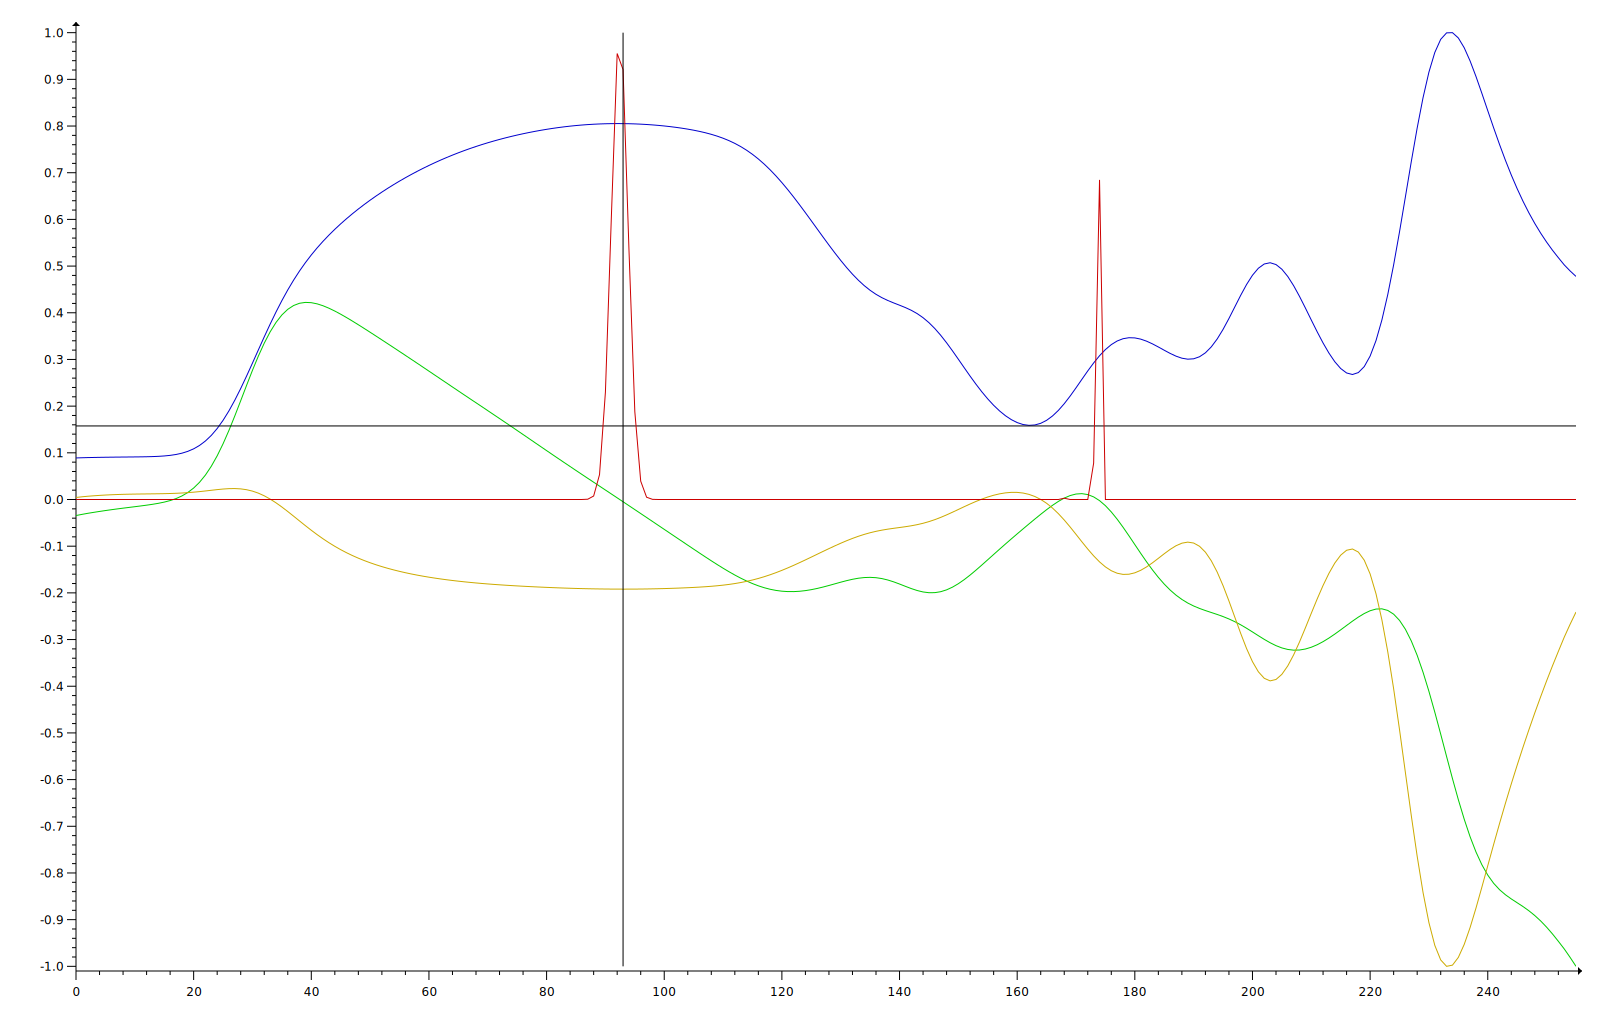
\includegraphics[width=0.35\textwidth]{images/r_g_3sphere}
		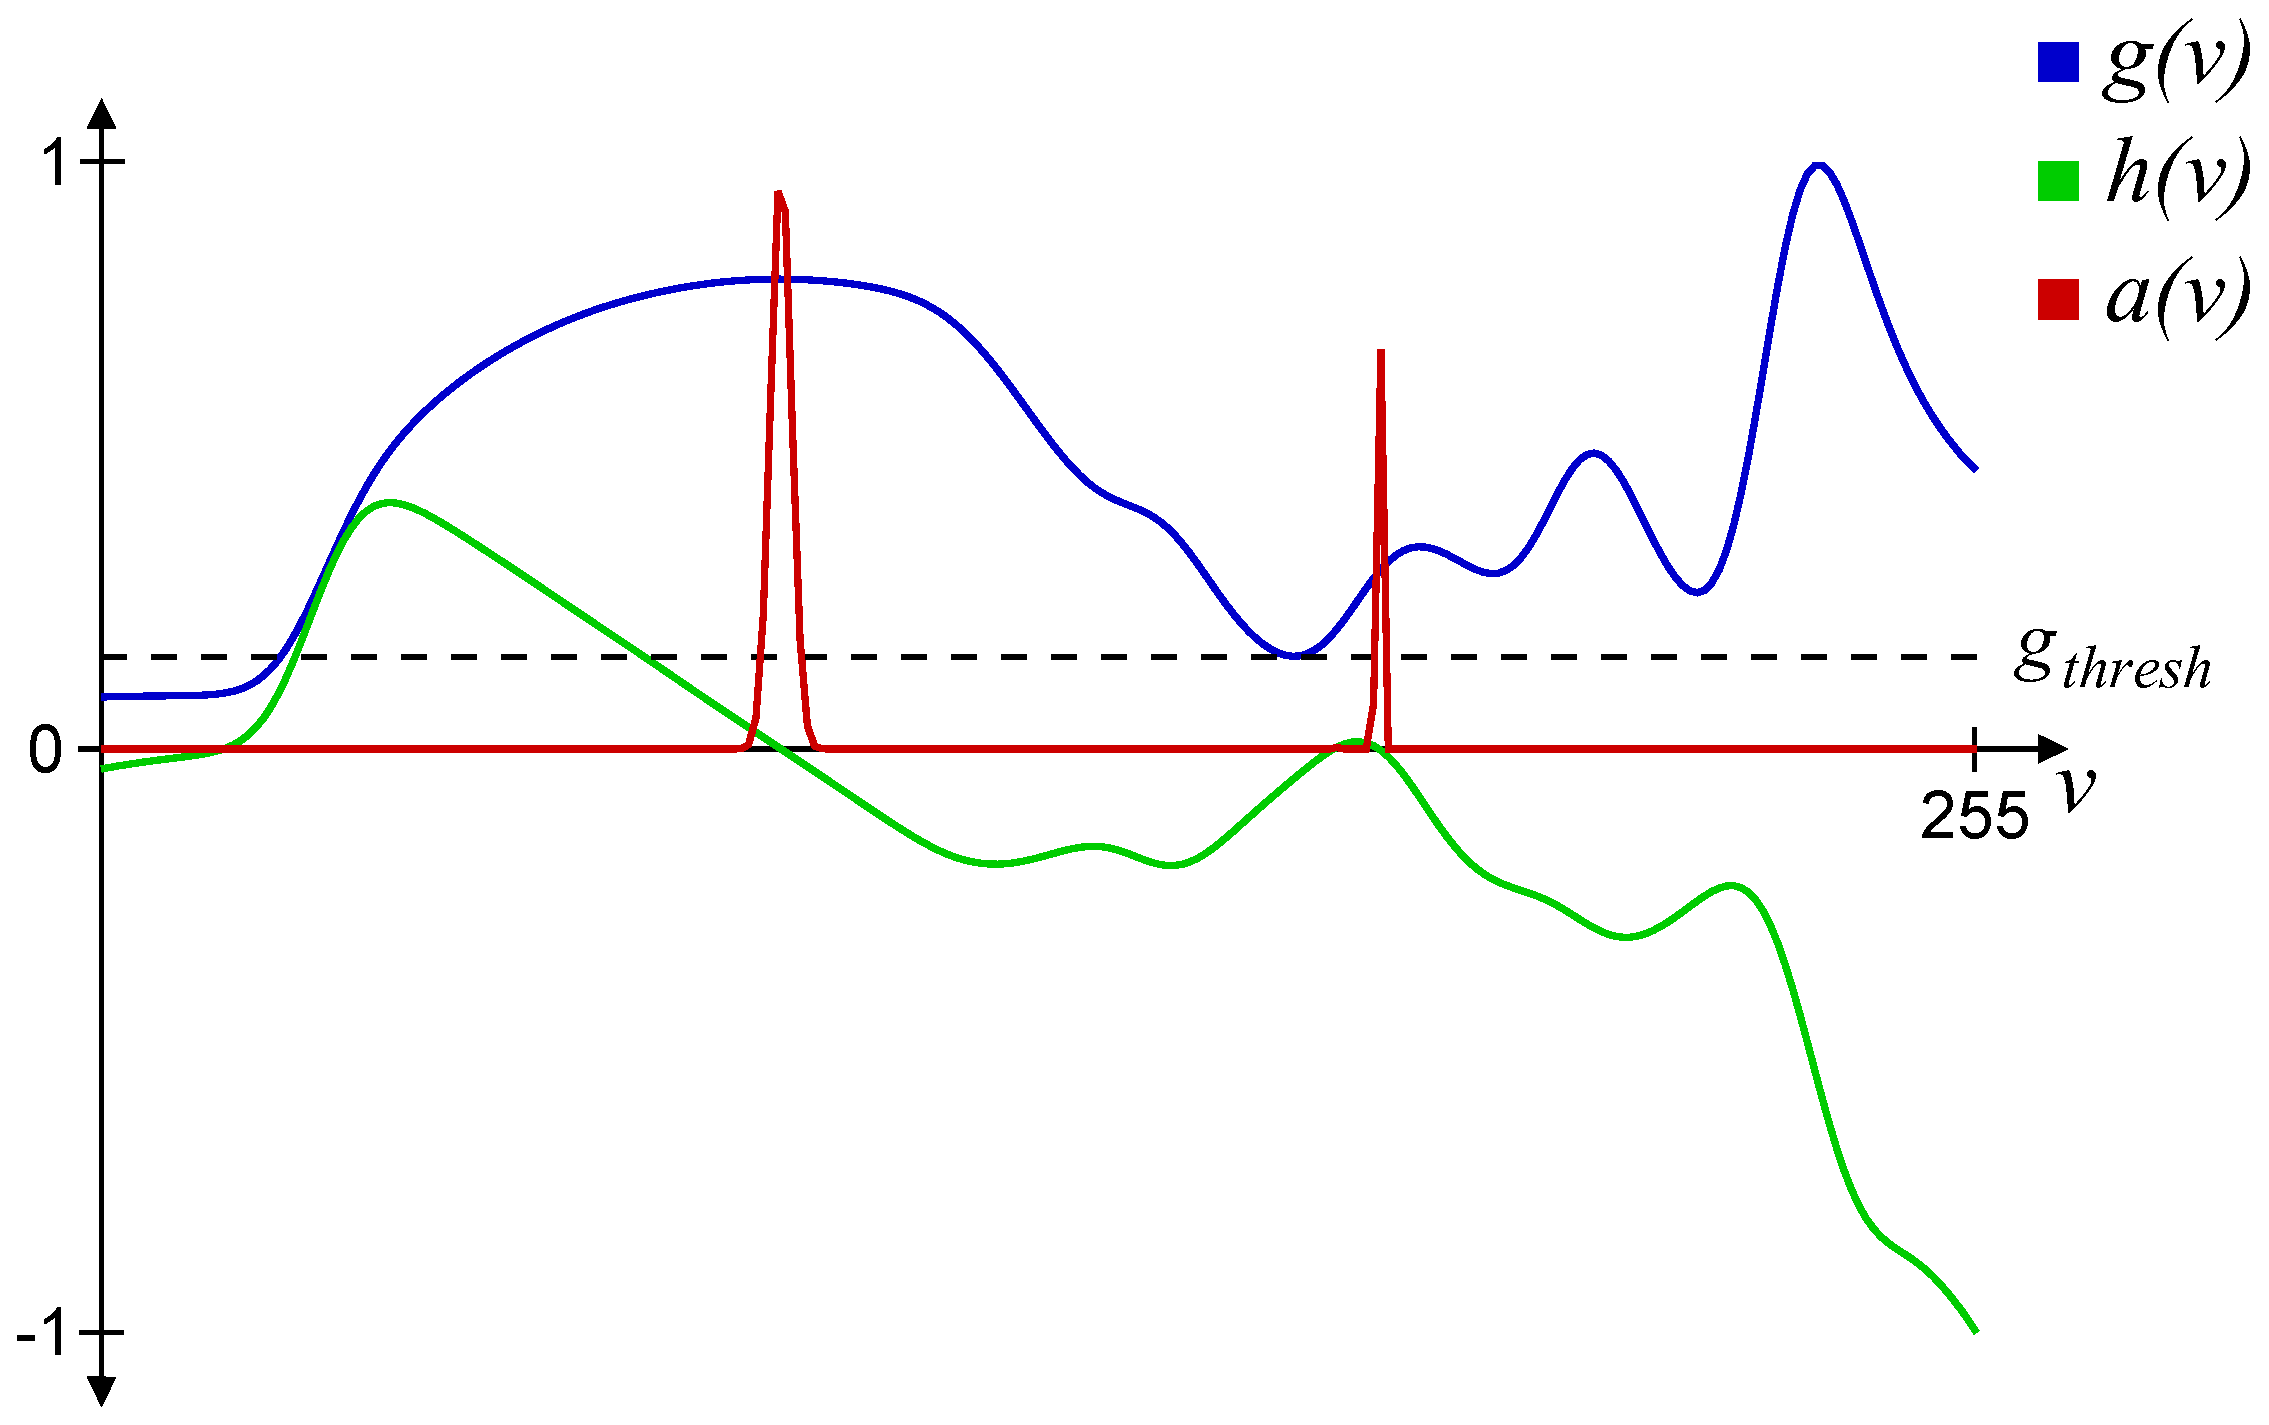
\includegraphics[width=0.65\textwidth]{images/r_g_3sphere_ft}
		\label{fig:r_3sphere_kd}
	}
	\subfigure[Método proposto.]
	{
		\includegraphics[width=0.35\textwidth]{images/r_m_3sphere}
		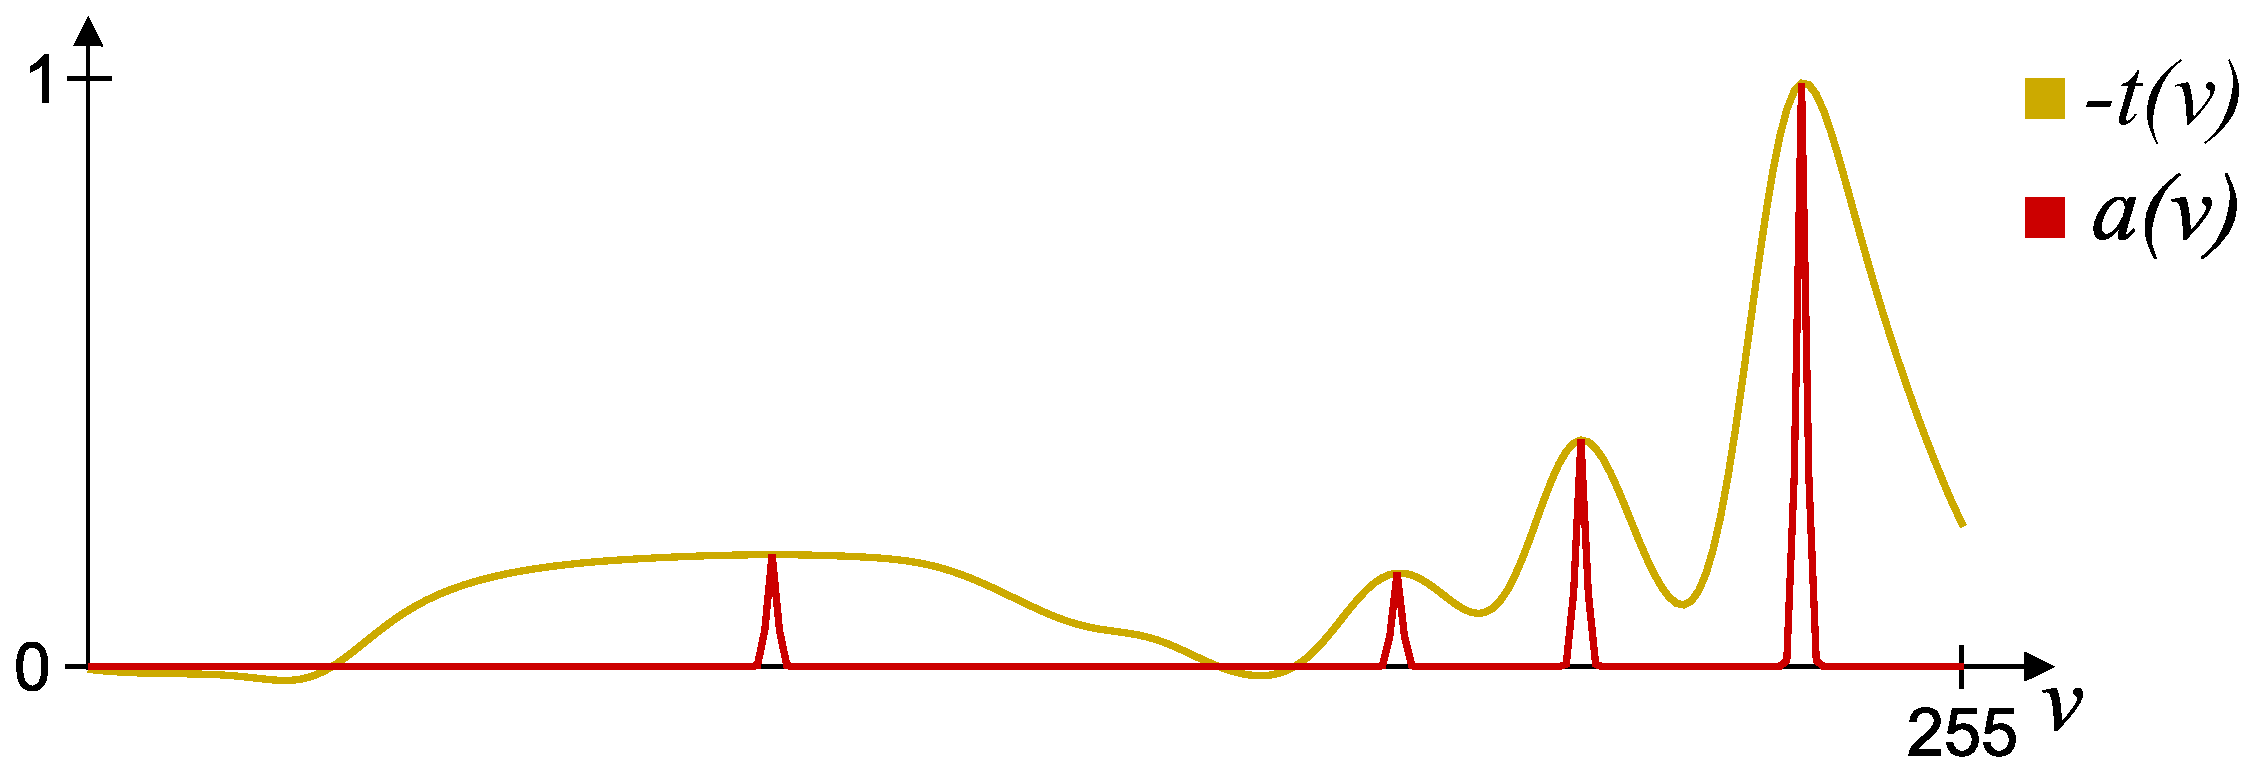
\includegraphics[width=0.65\textwidth]{images/r_m_3sphere_ft}			\label{fig:r_3sphere_mine}
	}
	\caption{Visualização e função de transferência do volume \quote{Test Spheres}.}
	\label{fig:r_3sphere}
\end{figure}

	A Figura~\ref{fig:r_3sphere} mostra que o método de \textit{Kindlmann e Durkin} apenas identifica $ 4 $ esferas. Conhecendo a escala de cores sabe-se que, na Figura~\ref{fig:r_3sphere}~\ref{fig:r_3sphere_kd}, o primeiro pico da FT corresponde à esfera mais externa, de cor verde, enquanto o segundo corresponde às outras, de tom alaranjado. No entanto, se apenas um pico realçou 3 fronteiras e há uma grande variação em sua opacidade conclui-se que a esfera menos opaca apenas foi capturada devido à sobreposição de intervalos. Na verdade, o método não a detectou. Jà o método proposto por esta dissertação identificou corretamente todas as esferas, como mostra a Figura~\ref{fig:r_3sphere}~\ref{fig:r_3sphere_mine}

%%%%%%%%%%%%%%%%%%%%%%%%%%%%%%%%%% NUCLEON %%%%%%%%%%%%%%%%%%%%%%%%%%%%%%%%%%%%%
\begin{figure}[h]
	\centering
	\includegraphics[width=0.25\textwidth]{images/g_nucleon_slice}
	\caption{Fatia do volume \quote{Nucleon}.}
	\label{fig:r_nucleon_slice}
\end{figure}

\begin{figure}[t]
	\centering
	\subfigure[Método de \textit{Kindlmann e Durkin}.]
	{
		\includegraphics[width=0.35\textwidth]{images/g_nucleon}
		\includegraphics[width=0.65\textwidth]{images/r_g_nucleon_ft}
		\label{fig:r_nucleon_kd}
	}
	\subfigure[Método proposto.]
	{
		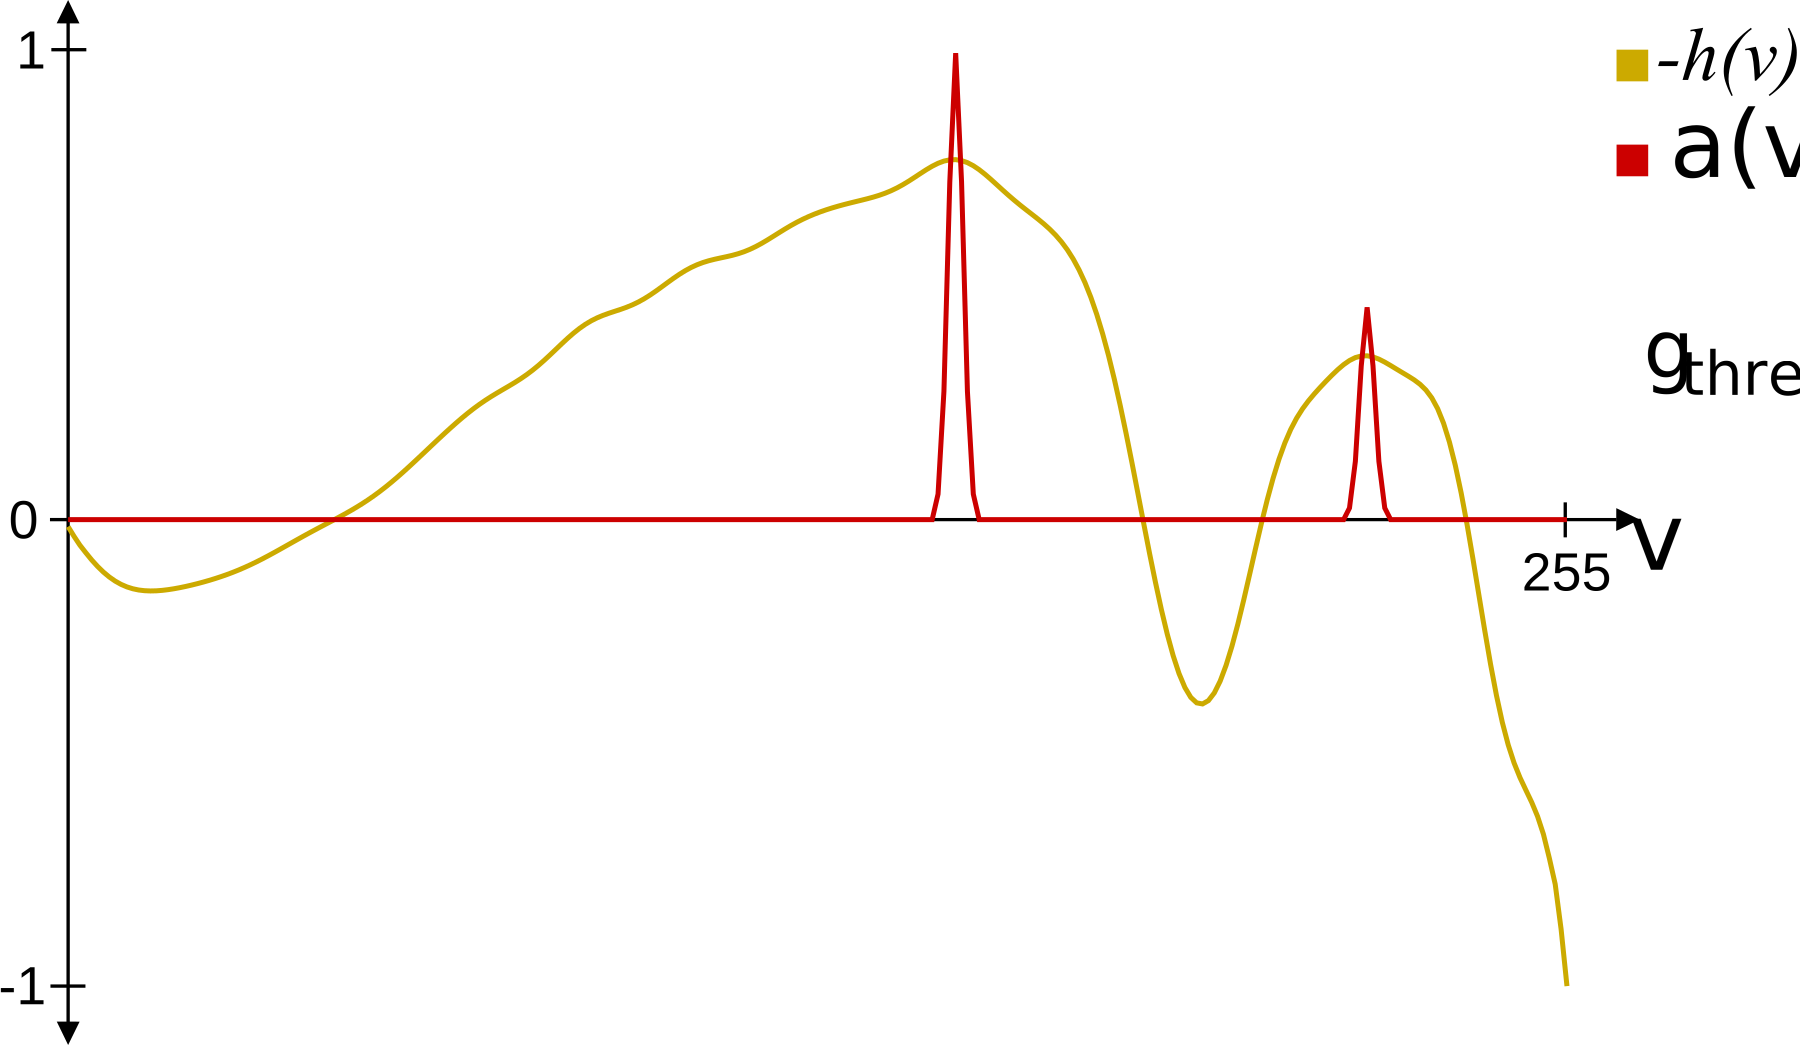
\includegraphics[width=0.35\textwidth]{images/r_m_nucleon}
		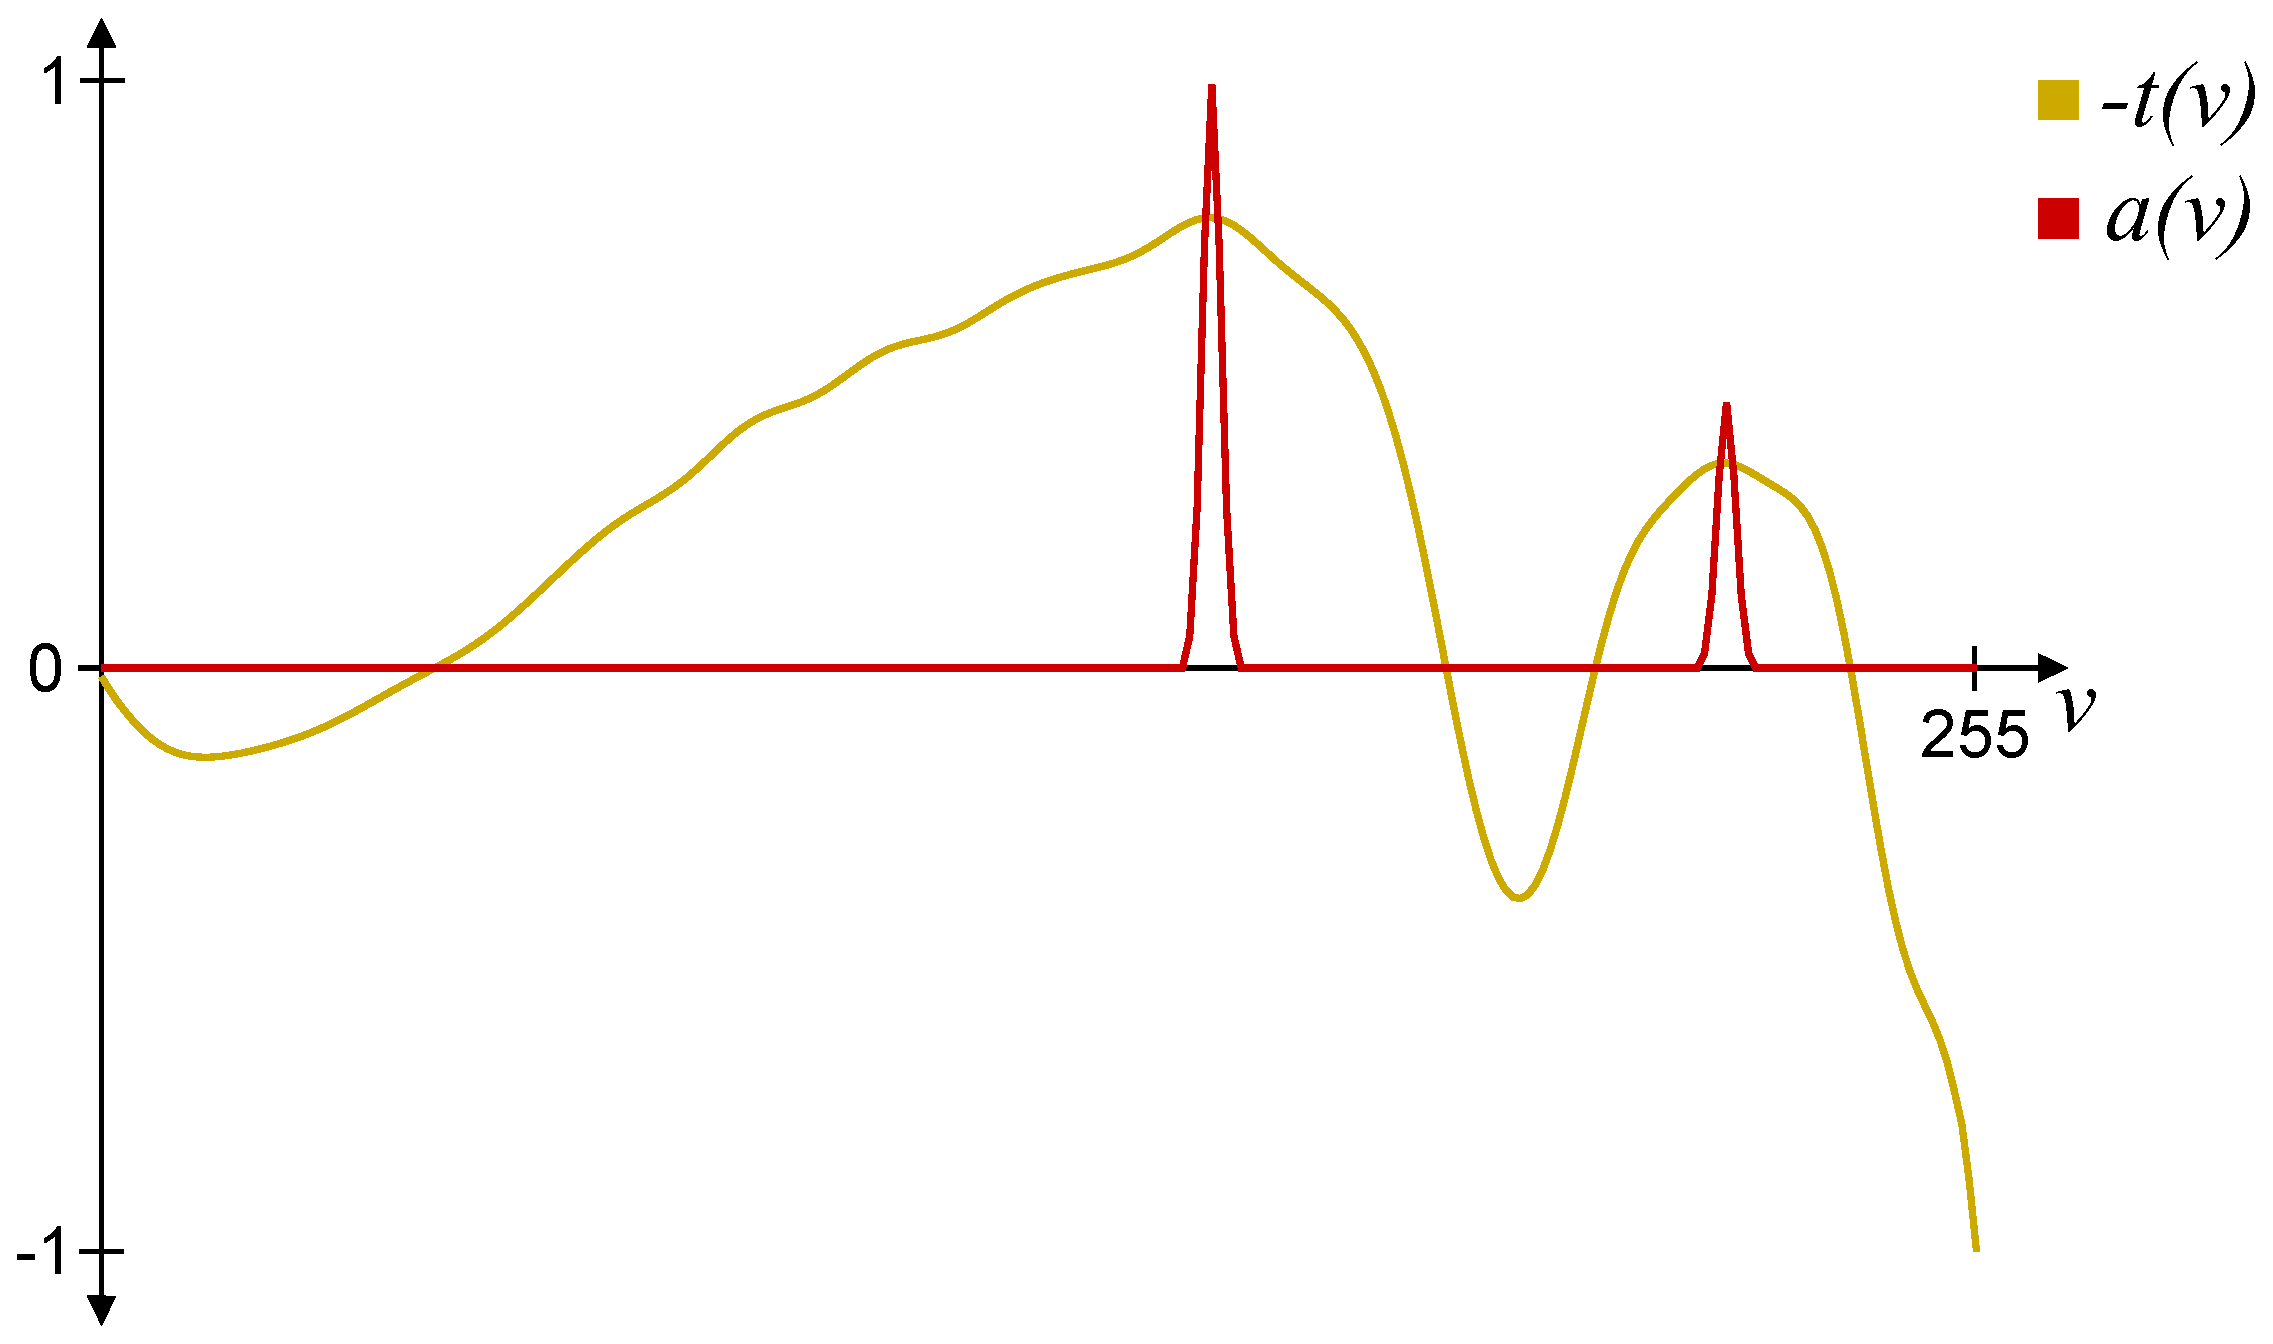
\includegraphics[width=0.65\textwidth]{images/r_m_nucleon_ft}			\label{fig:r_nucleon_mine}
	}
	\caption{Visualização e função de transferência do volume \quote{Nucleon}.}
	\label{fig:r_nucleon}
\end{figure}

A Figura~\ref{fig:r_nucleon} mostra mais um caso em que o método de \textit{Kindlmann e Durkin} não identifica todas as fronteiras existentes. Através da fatia do volume \quote{Nucleon}, exibida na Figura~\ref{fig:r_nucleon_slice}, vê-se que existem 2 fronteiras: cinza-preto e branco-preto. Porém, como ilustra a Figura~\ref{fig:r_nucleon}~\ref{fig:r_nucleon_kd}, apenas uma fronteira é realçada: a equivalente à transição cinza-preto na fatia do volume. Já o método proposto nesta dissertação identifica corretamente as duas fronteiras, como mostra a Figura~\ref{fig:r_nucleon}~\ref{fig:r_nucleon_mine}.
	
%%%%%%%%%%%%%%%%%%%%%%%%%%%%%%%%%% ENGINE %%%%%%%%%%%%%%%%%%%%%%%%%%%%%%%%%%%%%
\begin{figure}[h]
	\centering
	\includegraphics[width=0.3\textwidth]{images/r_engine_slice}
	\caption{Fatia do volume \quote{Engine}.}
	\label{fig:r_engine_slice}
\end{figure}

\begin{figure}[t]
	\centering
	\subfigure[Método de \textit{Kindlmann e Durkin}.]
	{
		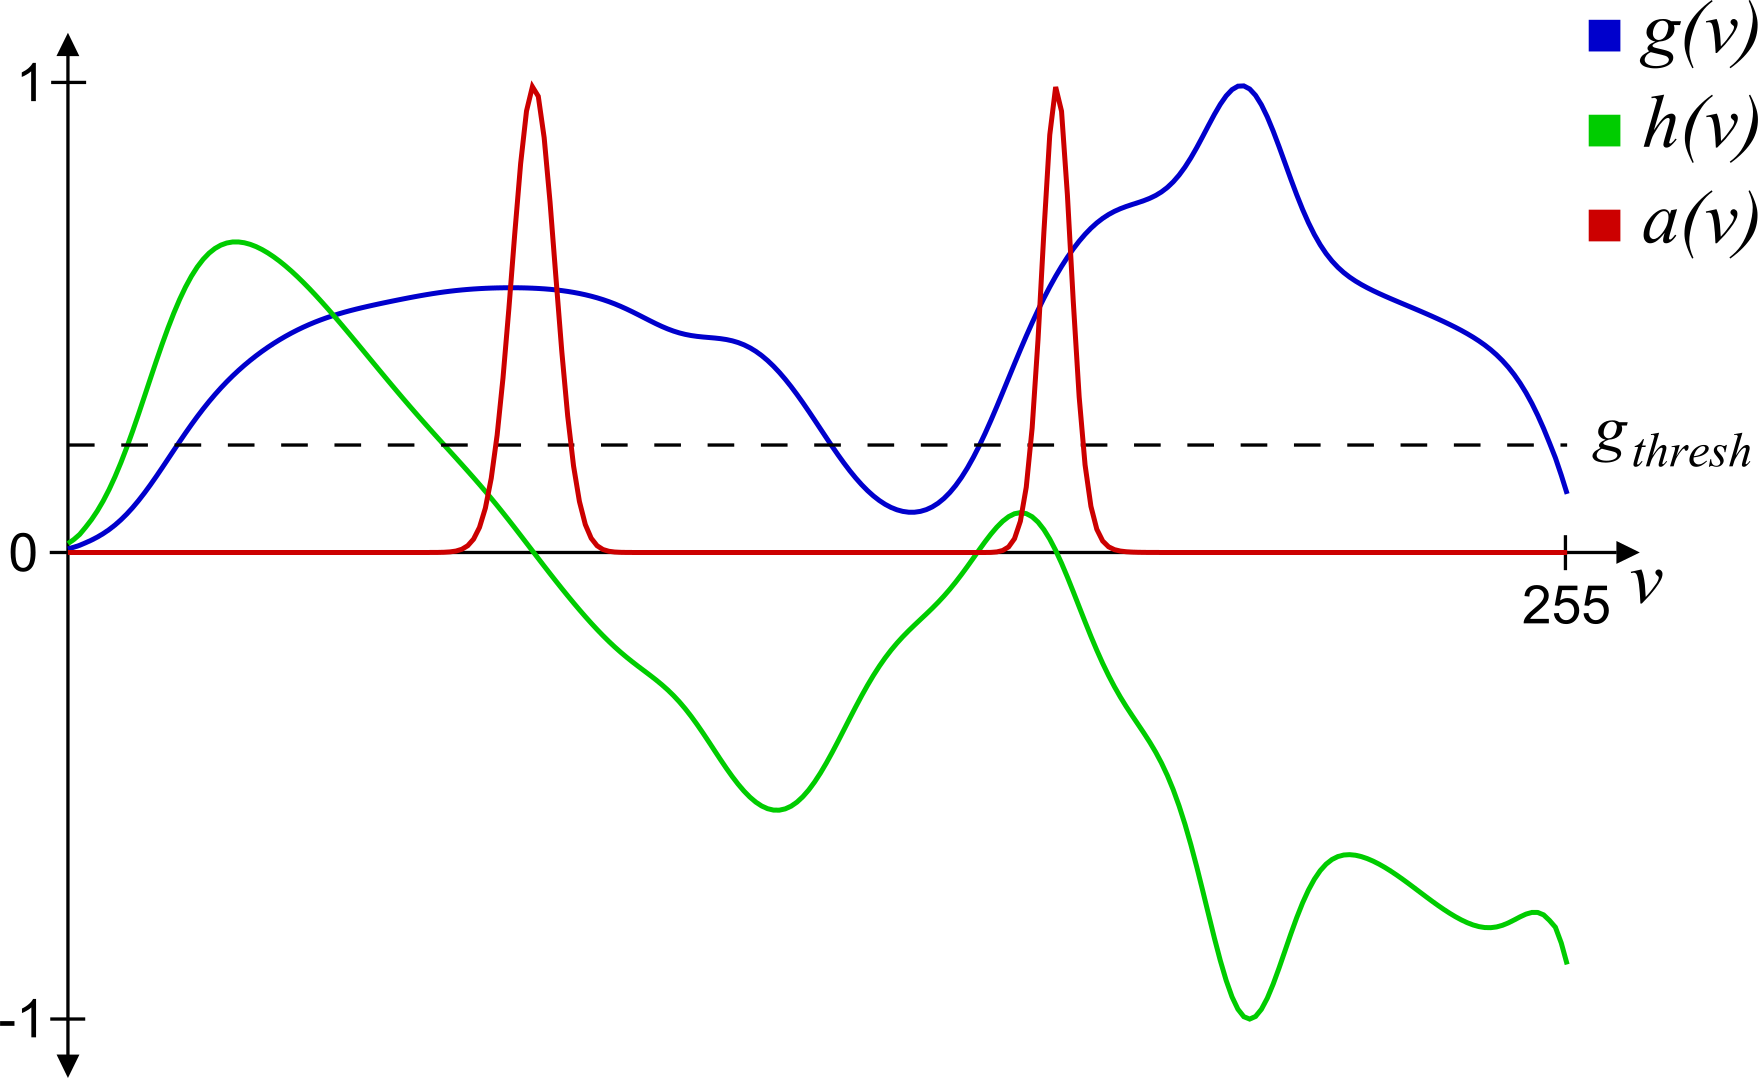
\includegraphics[width=0.35\textwidth]{images/r_g_engine}
		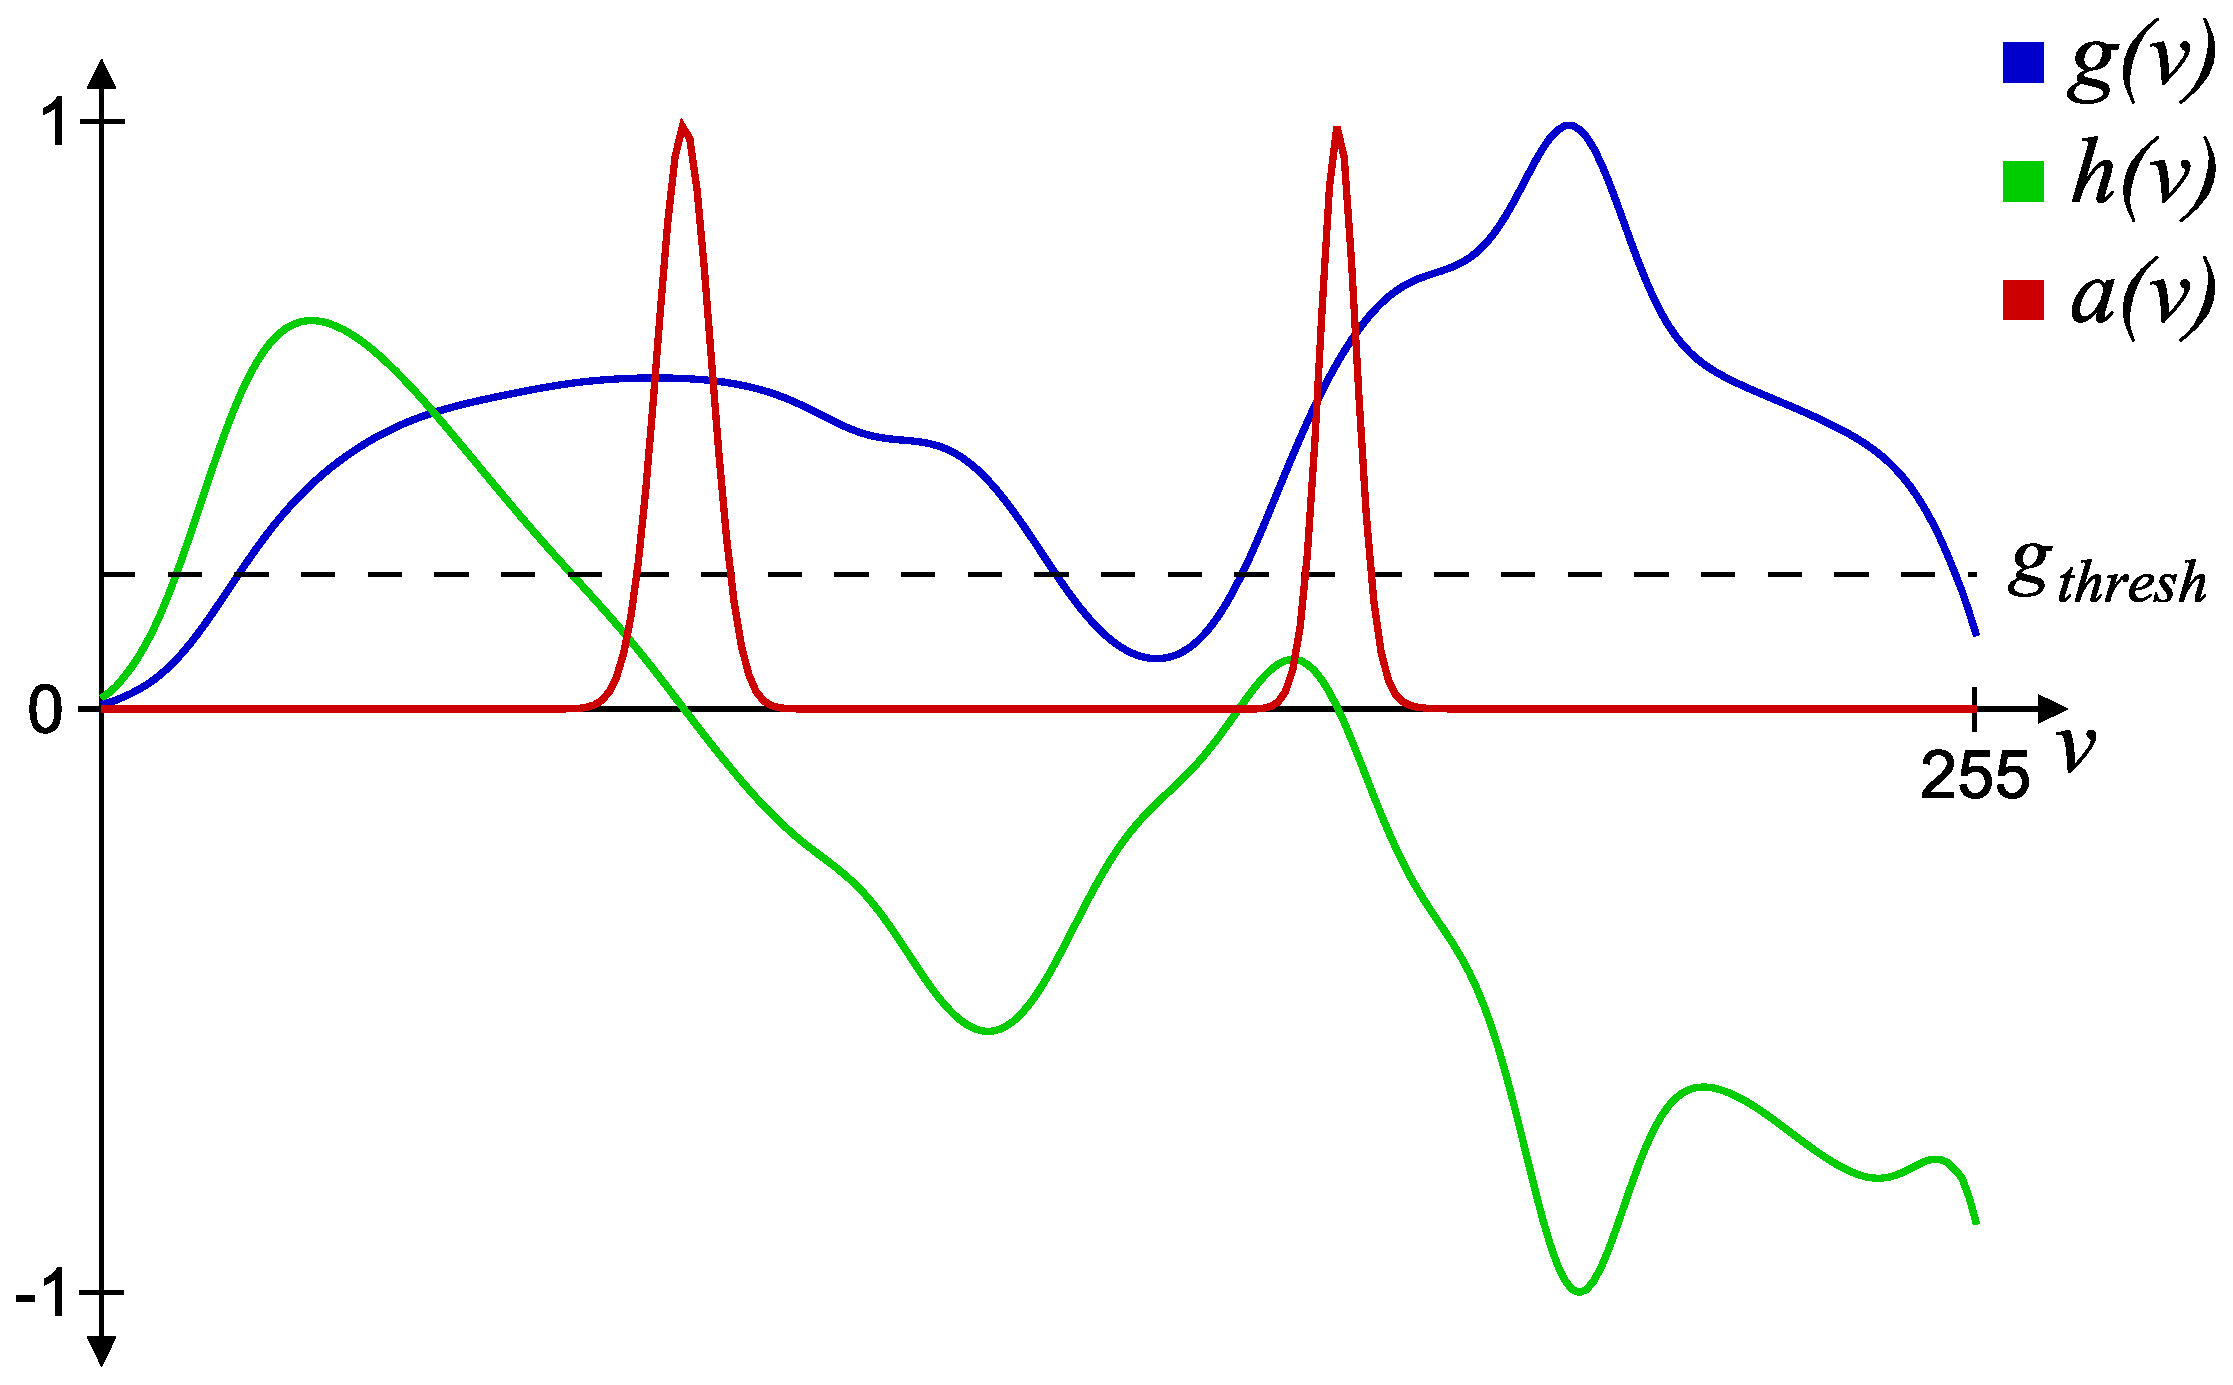
\includegraphics[width=0.65\textwidth]{images/r_g_engine_ft}
		\label{fig:r_engine_kd}
	}
	\subfigure[Método proposto.]
	{
		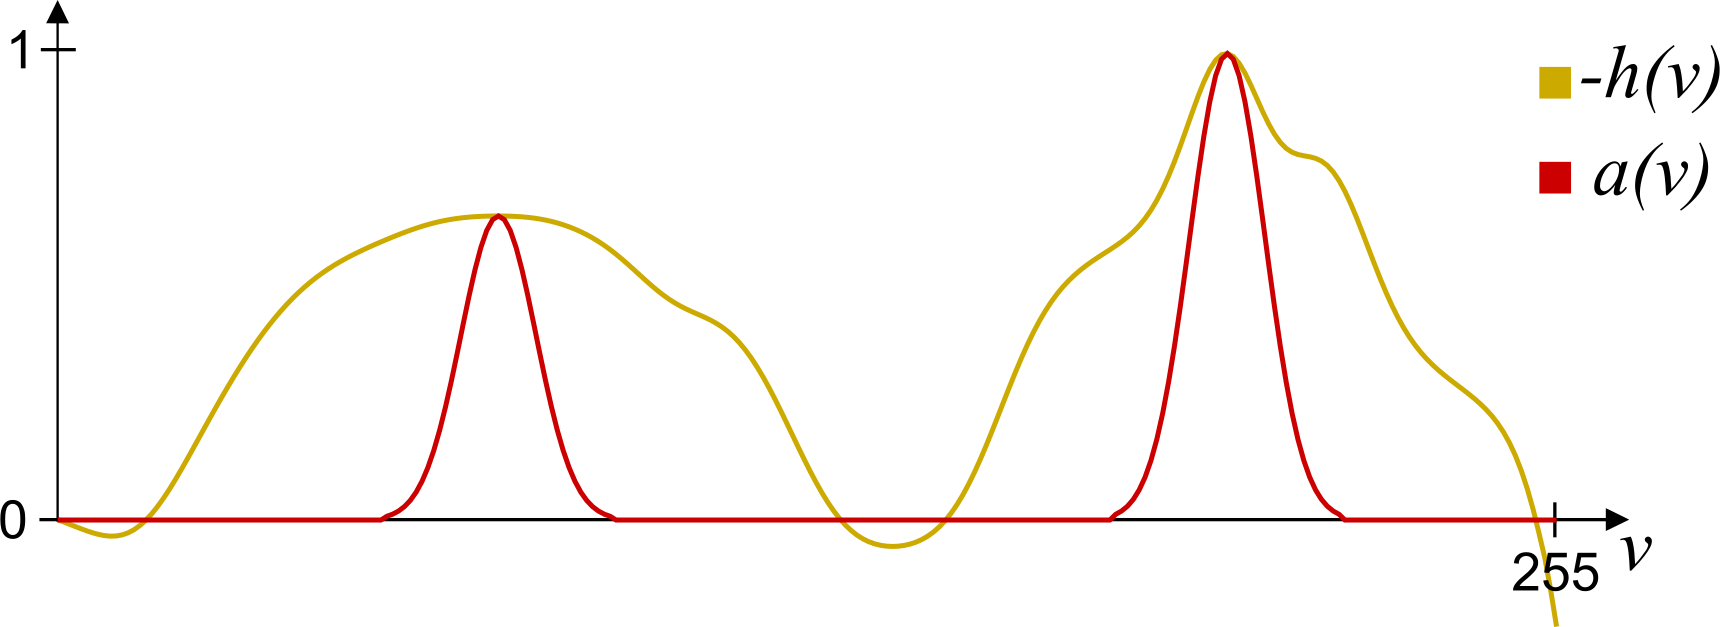
\includegraphics[width=0.35\textwidth]{images/r_m_engine}
		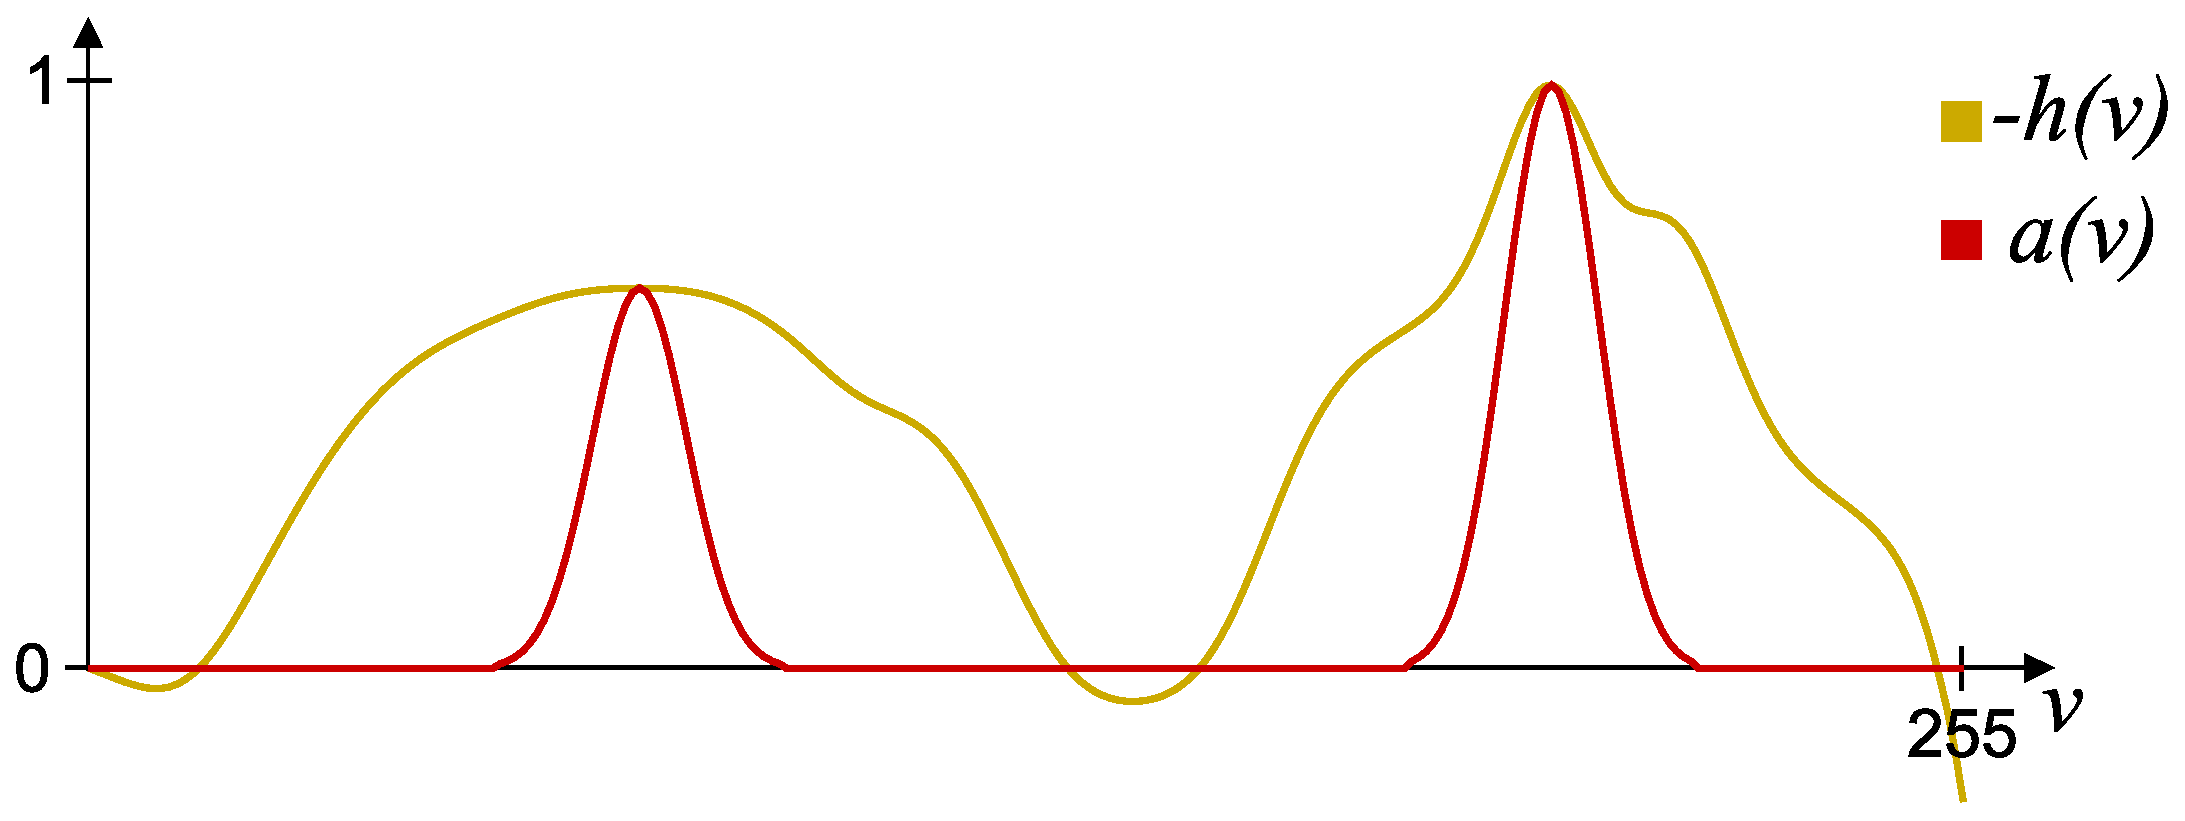
\includegraphics[width=0.65\textwidth]{images/r_m_engine_ft}			\label{fig:r_engine_mine}
	}
	\caption{Visualização e função de transferência do volume \quote{Engine}.}
	\label{fig:r_engine}
\end{figure}

A Figura~\ref{fig:r_engine_slice} exibe uma fatia do volume \quote{Engine}, onde pode ser observada a existência de $ 3 $ fronteiras. Comparando as visualizações resultantes dos dois métodos, exibidas na Figura~\ref{fig:r_engine}, percebe-se que ambos foram capazes de realçar corretamente as fronteiras do volume. No entanto, ressalta-se que esta equivalência só foi possível após encontrar o valor de $ g_{thresh} $ que eliminou algumas regiões da visualização do método de \textit{Kindlmann e Durkin} que foram realçadas indevidamente, devido ao deslocamento do segundo pico da sua função de transferência.
\clearpage
%%%%%%%%%%%%%%%%%%%%%%%%%%%%%%%%%% CT HEAD %%%%%%%%%%%%%%%%%%%%%%%%%%%%%%%%%%%%%
\begin{figure}[h]
	\centering
	\includegraphics[width=0.3\textwidth]{images/r_cthead_slice}
	\caption{Fatia do volume \quote{CT Head}.}
	\label{fig:r_cthead_slice}
\end{figure}

\begin{figure}[h]
	\centering
	\subfigure[Método de \textit{Kindlmann e Durkin}.]
	{
		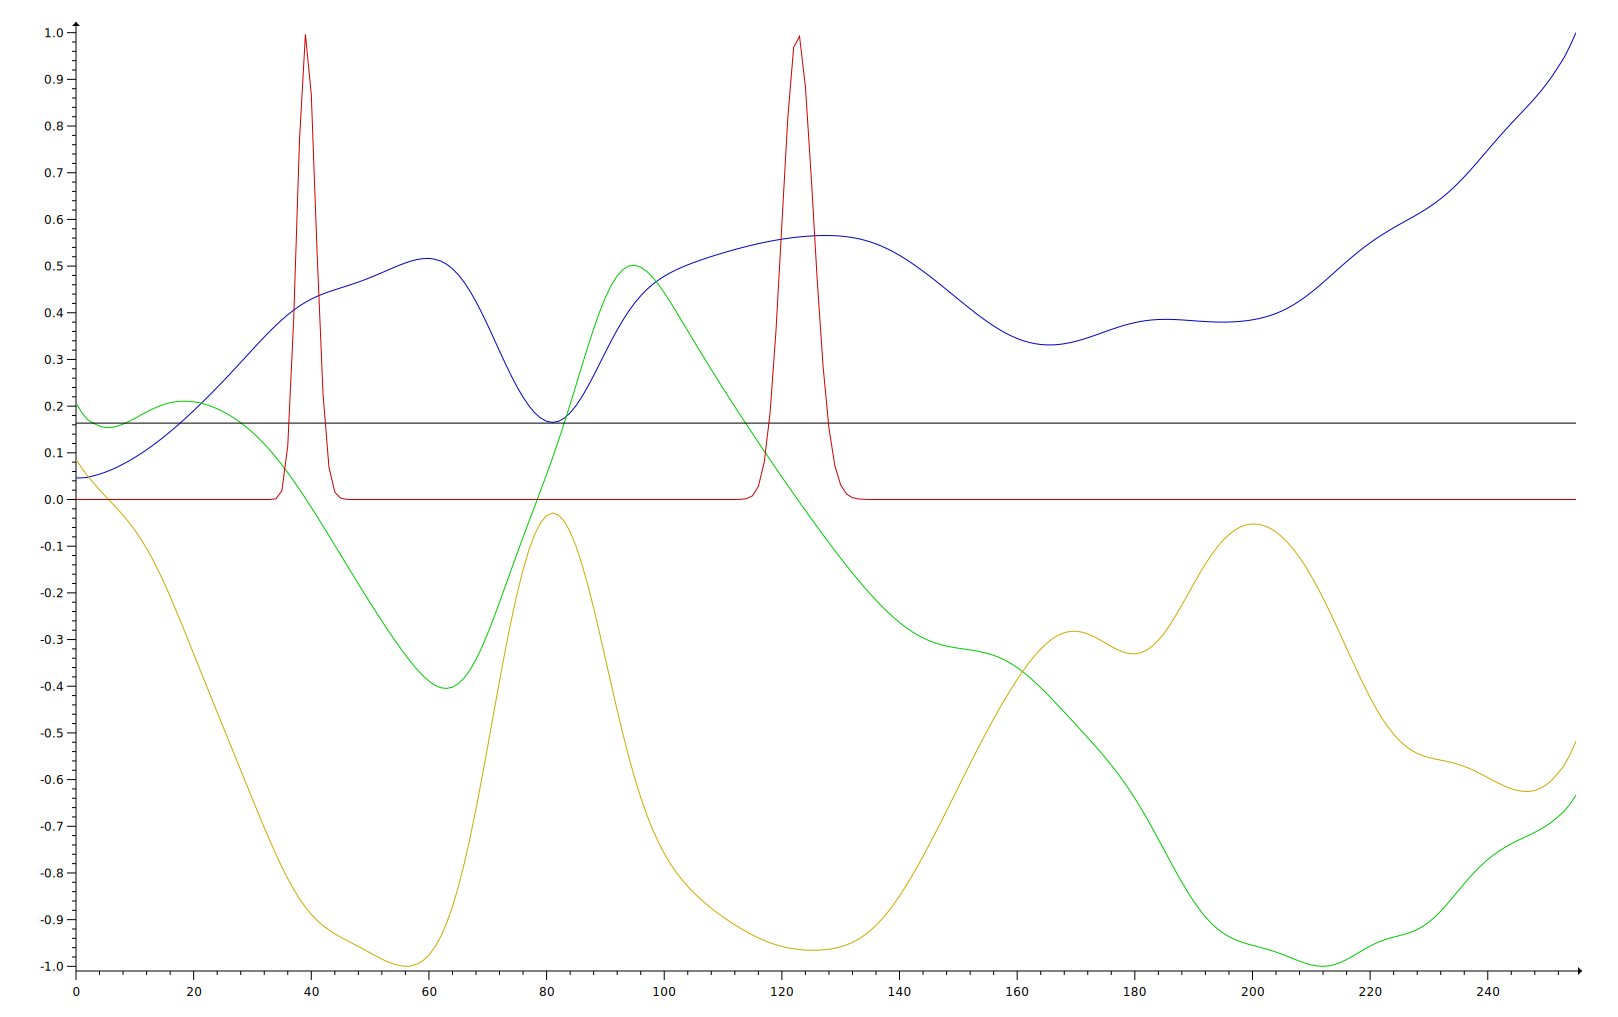
\includegraphics[width=0.35\textwidth]{images/r_g_cthead}
		\includegraphics[width=0.65\textwidth]{images/r_g_cthead_ft}
		\label{fig:r_cthead_kd}
	}
	\subfigure[Método proposto.]
	{
		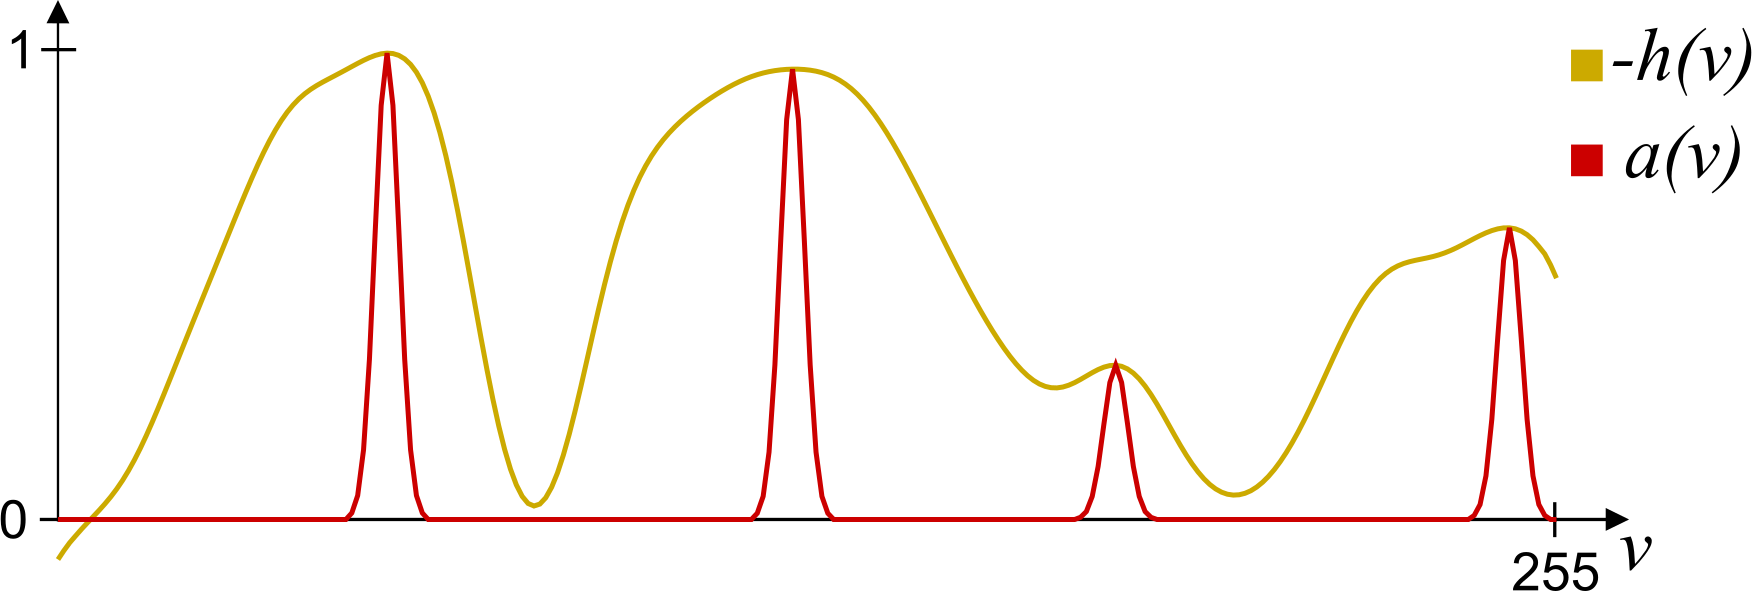
\includegraphics[width=0.35\textwidth]{images/r_m_cthead}
		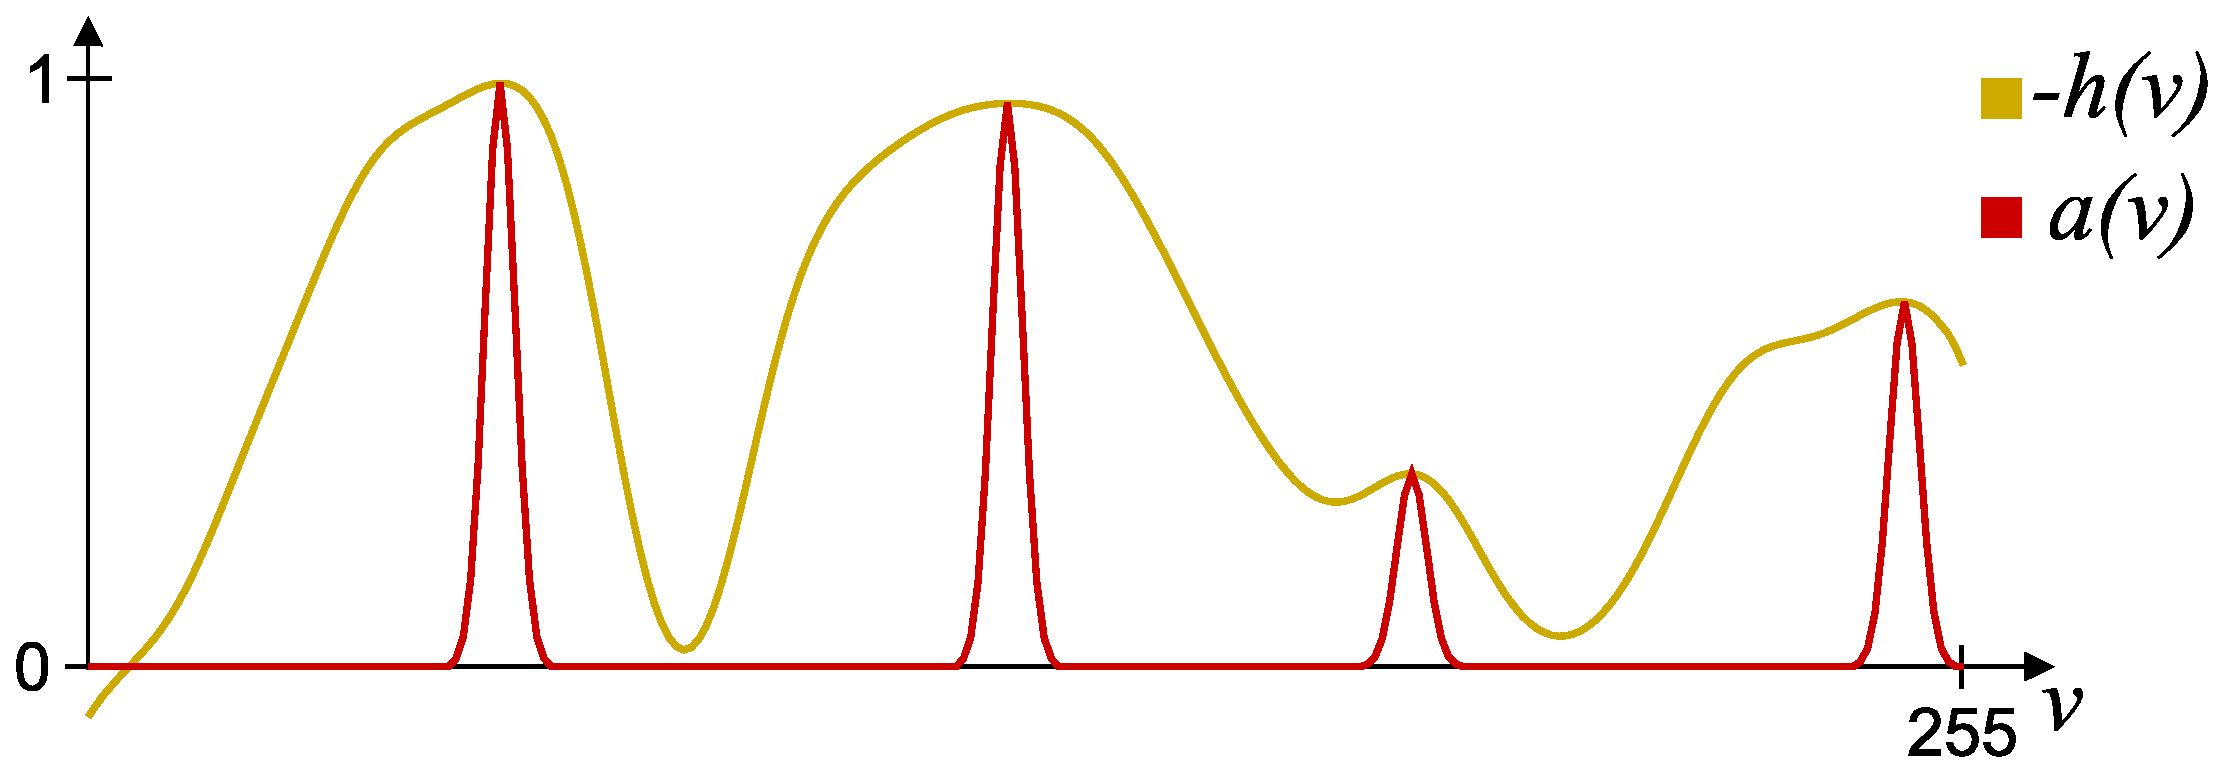
\includegraphics[width=0.65\textwidth]{images/r_m_cthead_ft}			\label{fig:r_cthead_mine}
	}
	\caption{Visualização e função de transferência do volume \quote{CT Head}.}
	\label{fig:r_cthead}
\end{figure}

	A Figura~\ref{fig:r_cthead_slice} apresenta uma fatia do volume \quote{CT Head}. Como pode ser observado, na parte de trás da cabeça do indivíduo, há uma estrutura que se comporta como uma fronteira. O método de \textit{Kindlmann e Durkin} realçou corretamente a cabeça e o crânio do indivíduo, bem como a estrutura comentada, como ilustra a Figura~\ref{fig:r_cthead}~\ref{fig:r_cthead_kd}. Jà o método proposto por esta dissertação foi capaz de realçar corretamente as fronteiras do indivíduo, porém, mostrando menos a estrutura presente na parte de trás. Este resultado, exibido na Figura~\ref{fig:r_cthead}~\ref{fig:r_cthead_mine} proporciona uma visualização mais limpa e, portanto, facilita ainda mais a compreensão do volume.

	Abaixo são exibidas as visualizações de alguns outros volumes conhecidos:
	
\begin{figure}[H]
	\centering
	\includegraphics[width=0.5\textwidth]{images/r_m_engine_iso}
	\caption{Estrutura interna do volume \quote{Engine}.}
\end{figure}

\begin{figure}[H]
	\centering
	\includegraphics[width=0.4\textwidth]{images/r_m_tooth}
	\caption{\quote{Tooth}.}
\end{figure}

\begin{figure}[H]
	\centering
	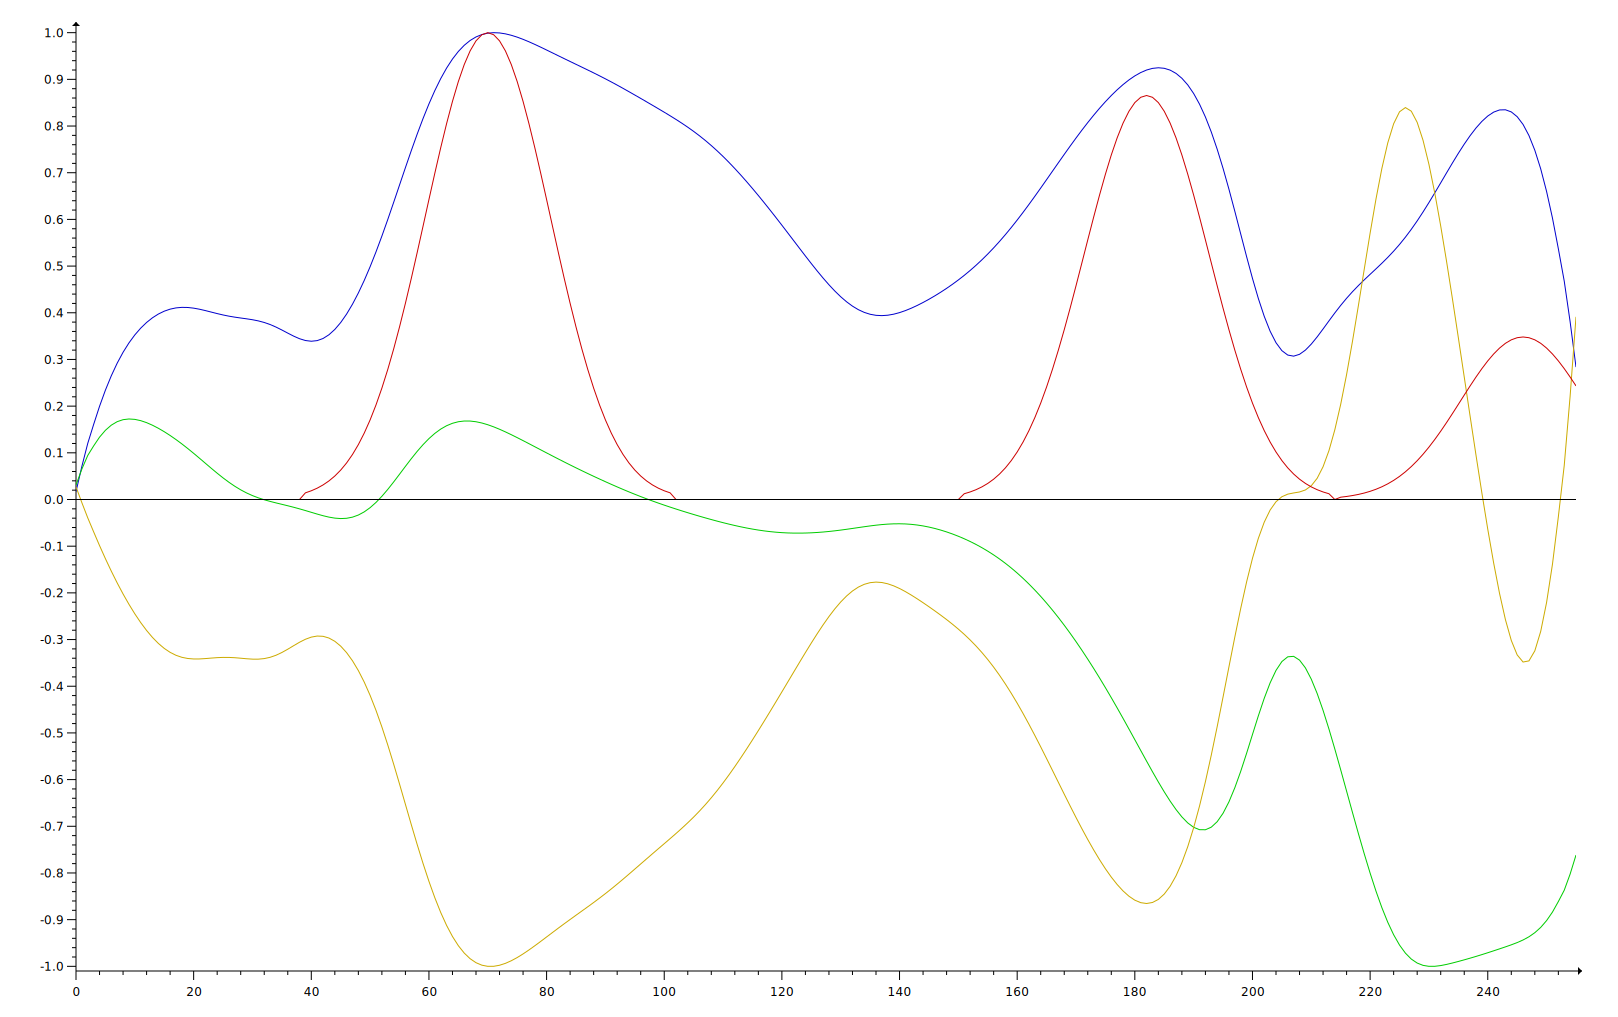
\includegraphics[width=0.8\textwidth]{images/r_m_bonsai}
	\caption{\quote{Bonsai}.}
\end{figure}

\begin{figure}[H]
	\centering
	\subfigure
	{
		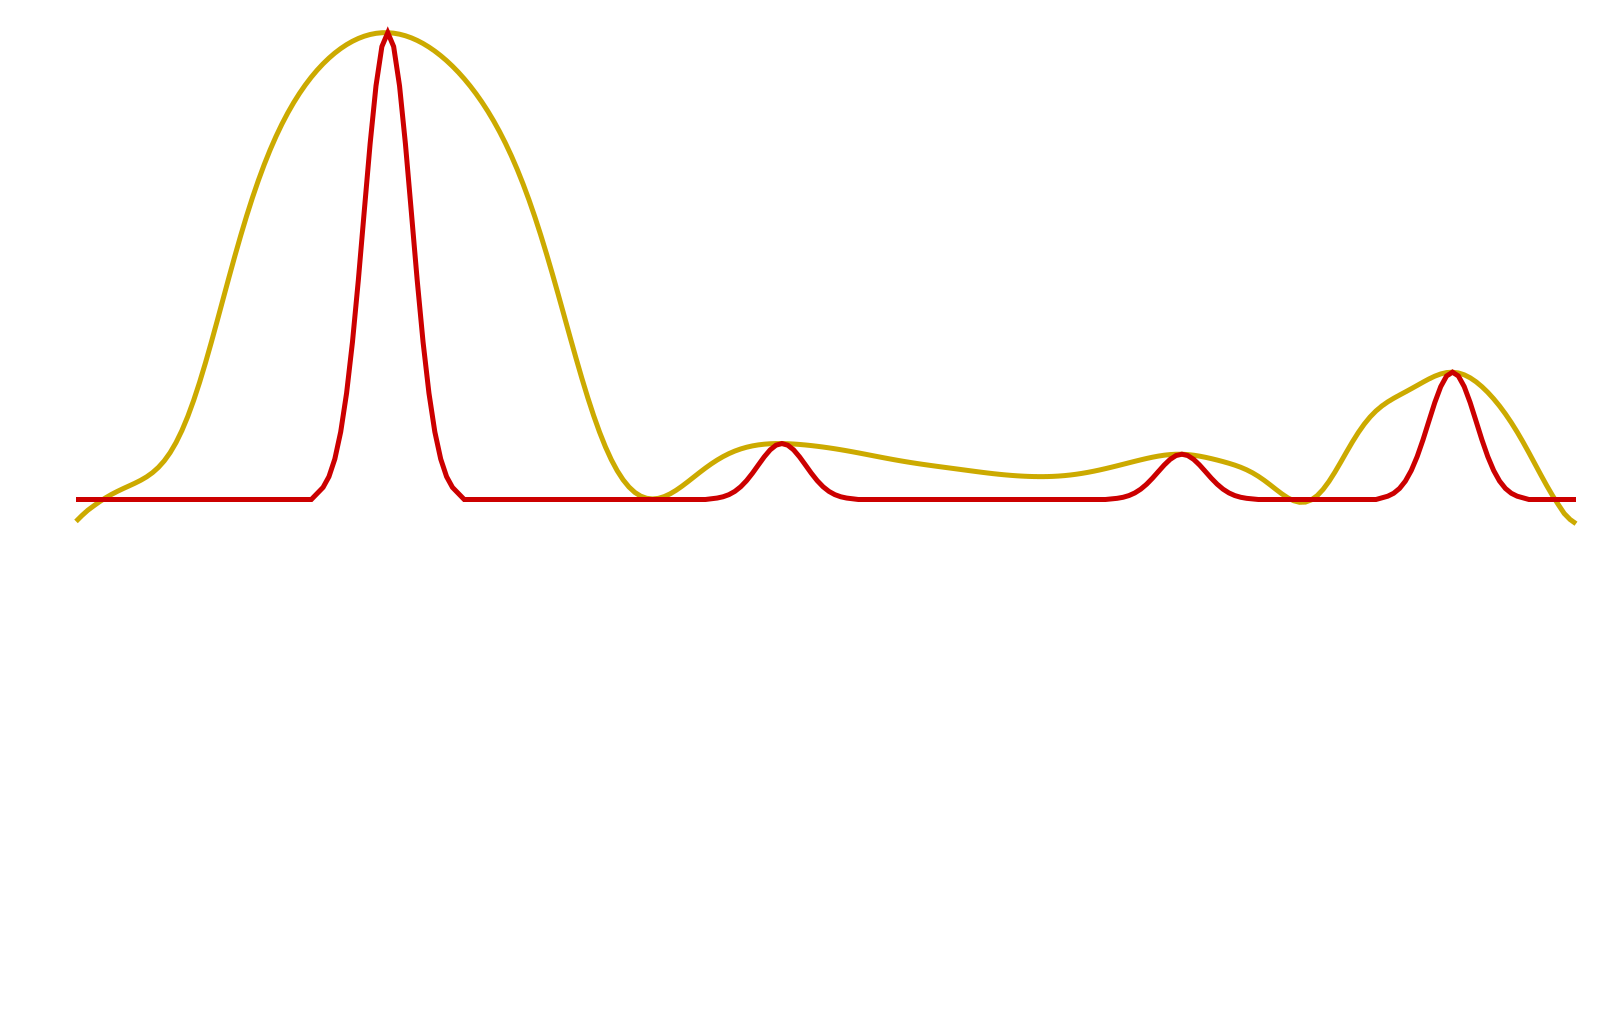
\includegraphics[width=0.7\textwidth]{images/r_m_carp}
	}
	\subfigure
	{
		\includegraphics[width=0.7\textwidth]{images/r_m_carp_up}
	}
	\subfigure
	{
		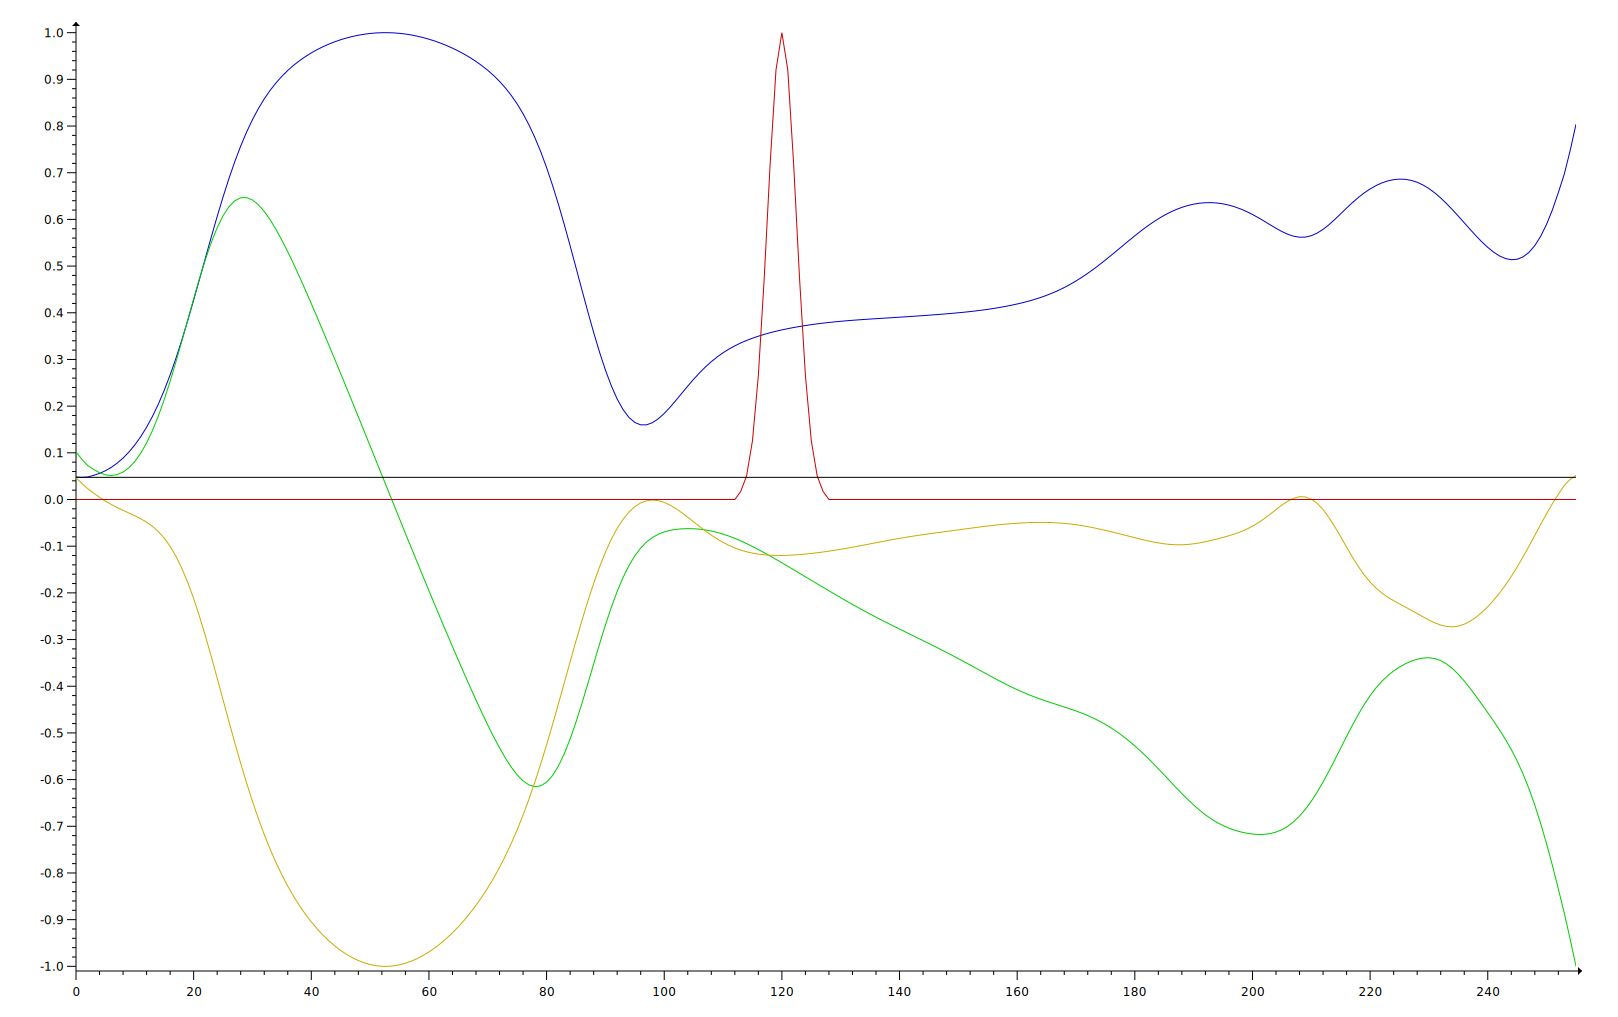
\includegraphics[width=0.7\textwidth]{images/r_m_carp_exo}
	}
	\caption{\quote{Carp}.}
\end{figure}

\begin{figure}[H]
	\centering
	\includegraphics[width=0.7\textwidth]{images/r_m_knee}
	\caption{\quote{Knee}.}
\end{figure}

\section{Malhas Não Regulares}
\label{sec:result.irreg}

	Para visualizar volumes com malhas não regulares foi preciso utilizar um outro visualizador. Escolheu-se então a técnica proposta por \textit{Miranda e Celes}~\cite{miranda} em \quote{Accurate volume rendering of unstructed hexahedral meshes}. Então, cinco volumes sintéticos no formato de um ortoedro são analisados. Esses volumes foram obtidos a partir de dois modelos de reservatório, chamados A e B, variando-se o time step da simulação ou a propriedade mapeada.
	
%%%%%%%%%%%%%%%%%%%%%%%%%%%%%%%%% VREP SO 1 %%%%%%%%%%%%%%%%%%%%%%%%%%%%%%%%%%%%
\begin{figure}[h]
	\centering
	\subfigure[]{
		\frame{\includegraphics[width=0.25\textwidth]{images/r_vrep_so_slice}}
	}
	\caption{Fatia do volume de SO do modelo A.}
	\label{fig:box_slice}
\end{figure}

	A figura acima mostra uma fatia do volume de saturação de óleo (SO) do modelo A, que possui um poço injetor no canto superior esquerdo e um produtor no canto diagonal oposto.

\begin{figure}[h]
	\centering
	\subfigure[Método de \textit{Kindlmann e Durkin}.]
	{
		\includegraphics[width=0.35\textwidth]{images/r_vrep_so_kd}
		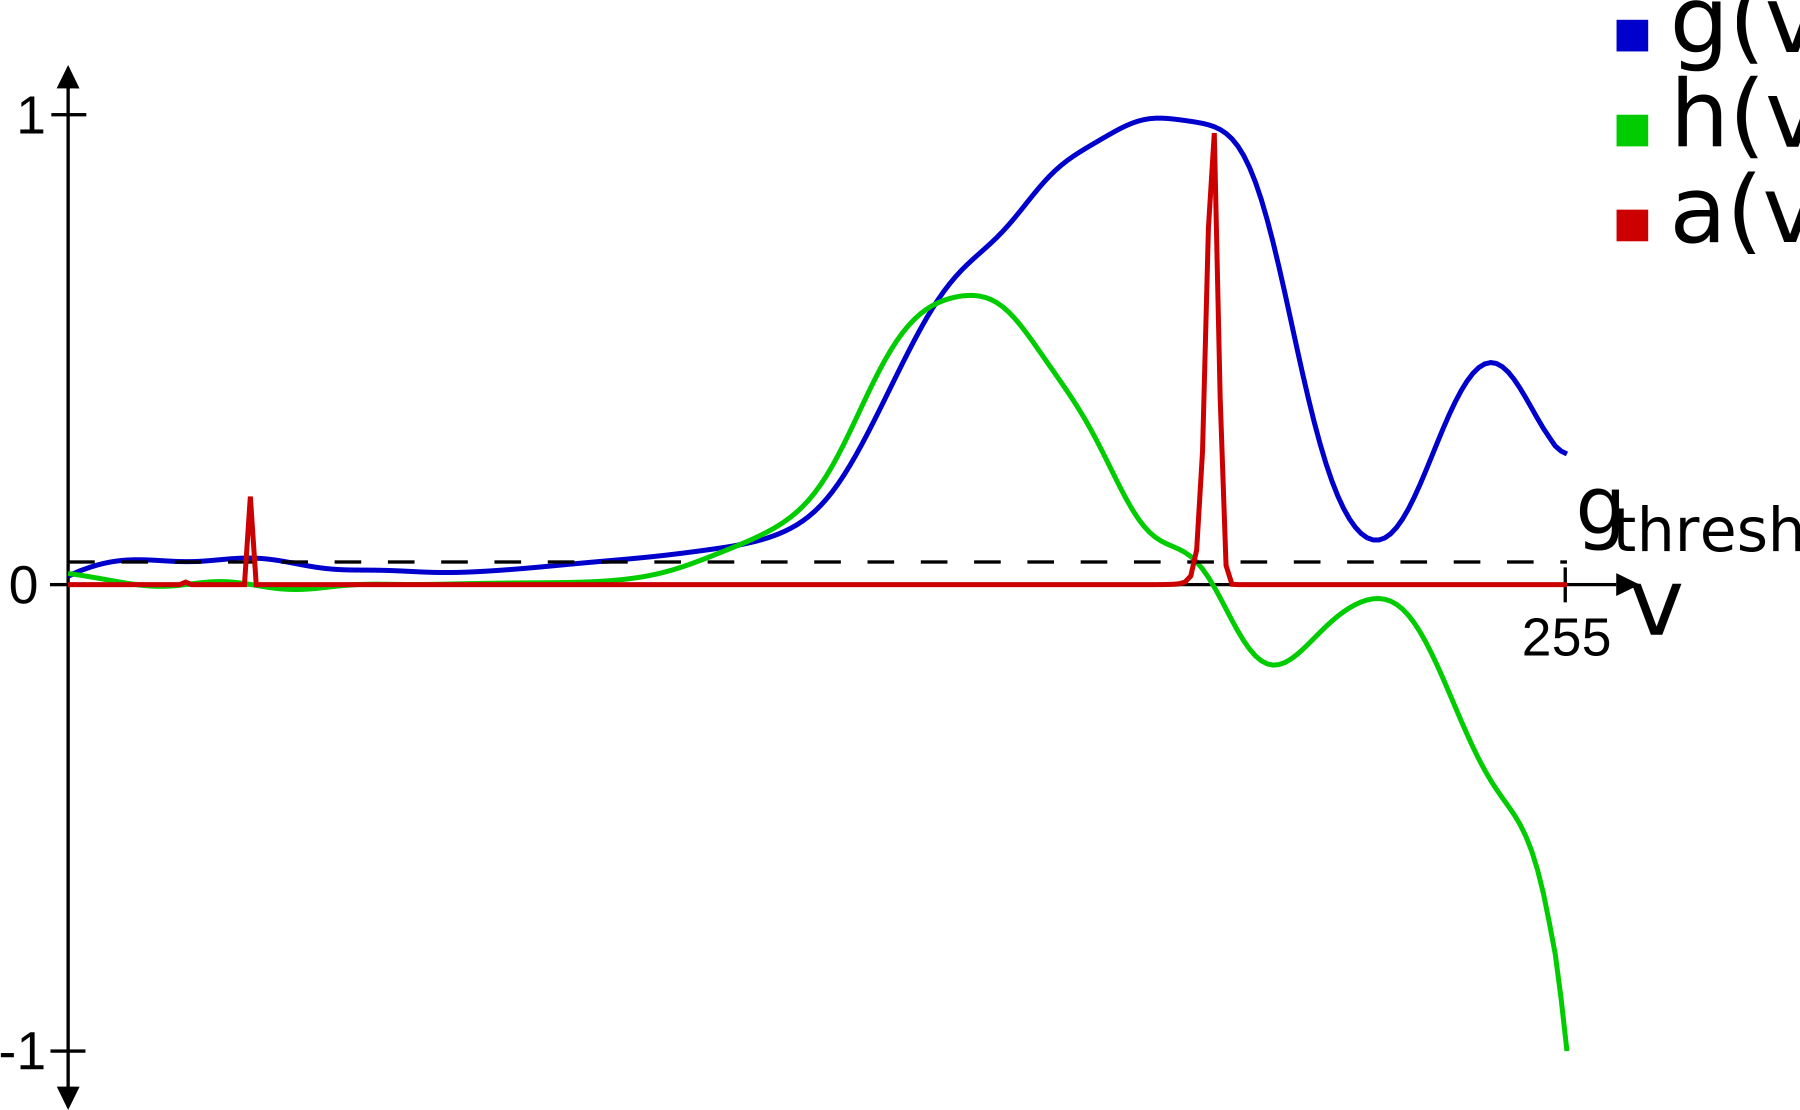
\includegraphics[width=0.65\textwidth]{images/r_vrep_so_kd_ft}
		\label{fig:r_vrep_kd}
	}
	\subfigure[Método proposto.]
	{
		\includegraphics[width=0.35\textwidth]{images/r_vrep_so_mine}
		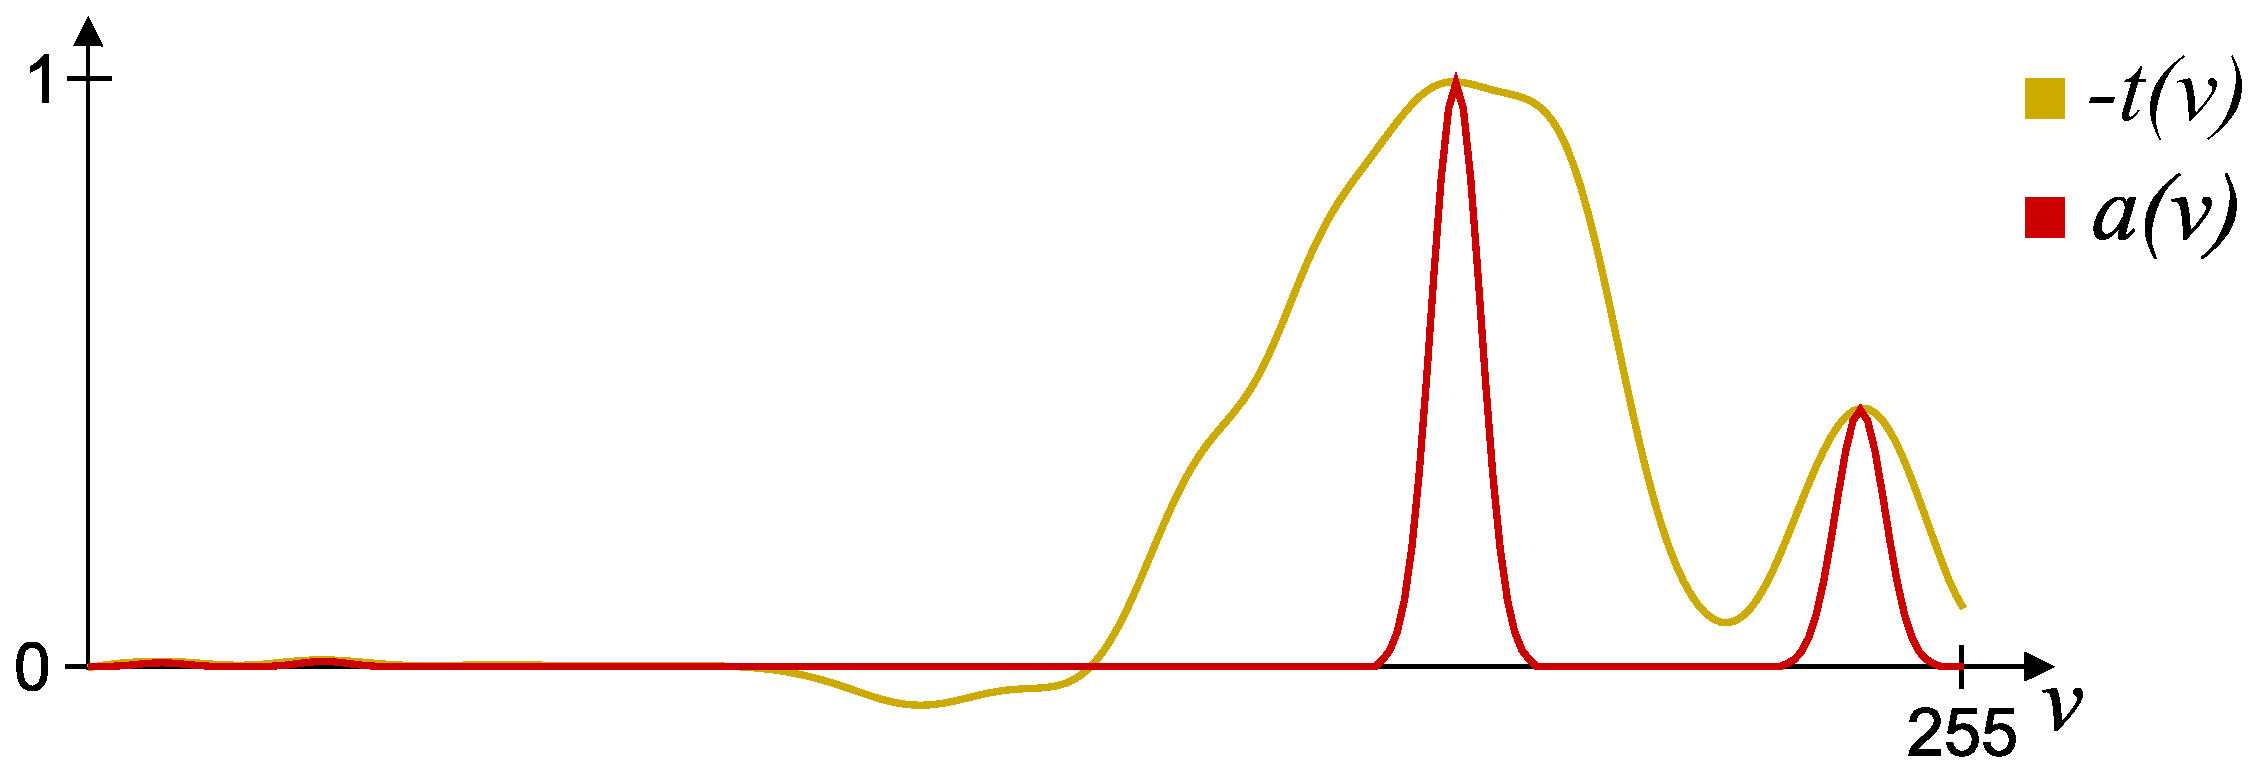
\includegraphics[width=0.65\textwidth]{images/r_vrep_so_mine_ft}			\label{fig:r_vrep_mine}
	}
	\caption{FT e visualização do volume de SO do modelo~A.}
	\label{fig:r_vrep}
\end{figure}

	Como pode ser visto na Figura~\ref{fig:box_slice}, o reservatório possui duas fronteiras bem destacadas e uma mais fraca que são, respectivamente: cinza escuro-branco, branco-cinza claro e preto-cinza escuro. A Figura~\ref{fig:r_vrep} mostra que o método de \textit{Kindlmann e Durkin} identifica apenas a primeira e a terceira das fronteiras listadas, reforçando o quanto essa abordagem é dependente de $ h(v) = 0 $. Já o método descrito por esta dissertação identifica uma fronteira fraca a mais que o esperado. Porém, realça corretamente as duas mais fortes.

%%%%%%%%%%%%%%%%%%%%%%%%%%%%%%%%% VREP SO 2 %%%%%%%%%%%%%%%%%%%%%%%%%%%%%%%%%%%%
\begin{figure}[h]
	\centering
	\frame{\includegraphics[width=0.3\textwidth]{images/r_vrep_so_2_slice_}}
	\caption{Fatia do volume de SO do modelo A.}
	\label{fig:r_vrep_2_slice}
\end{figure}

	A figura acima refere-se ao mesmo volume da Figura~\ref{fig:box_slice}, mas em outro momento da simulação. Agora há apenas uma fronteira forte (1) e três fracas (2, 3 e 4).

\begin{figure}[h]
	\centering
	\subfigure[Método de \textit{Kindlmann e Durkin}.]
	{
		\includegraphics[width=0.35\textwidth]{images/r_vrep_so_2_kd}
		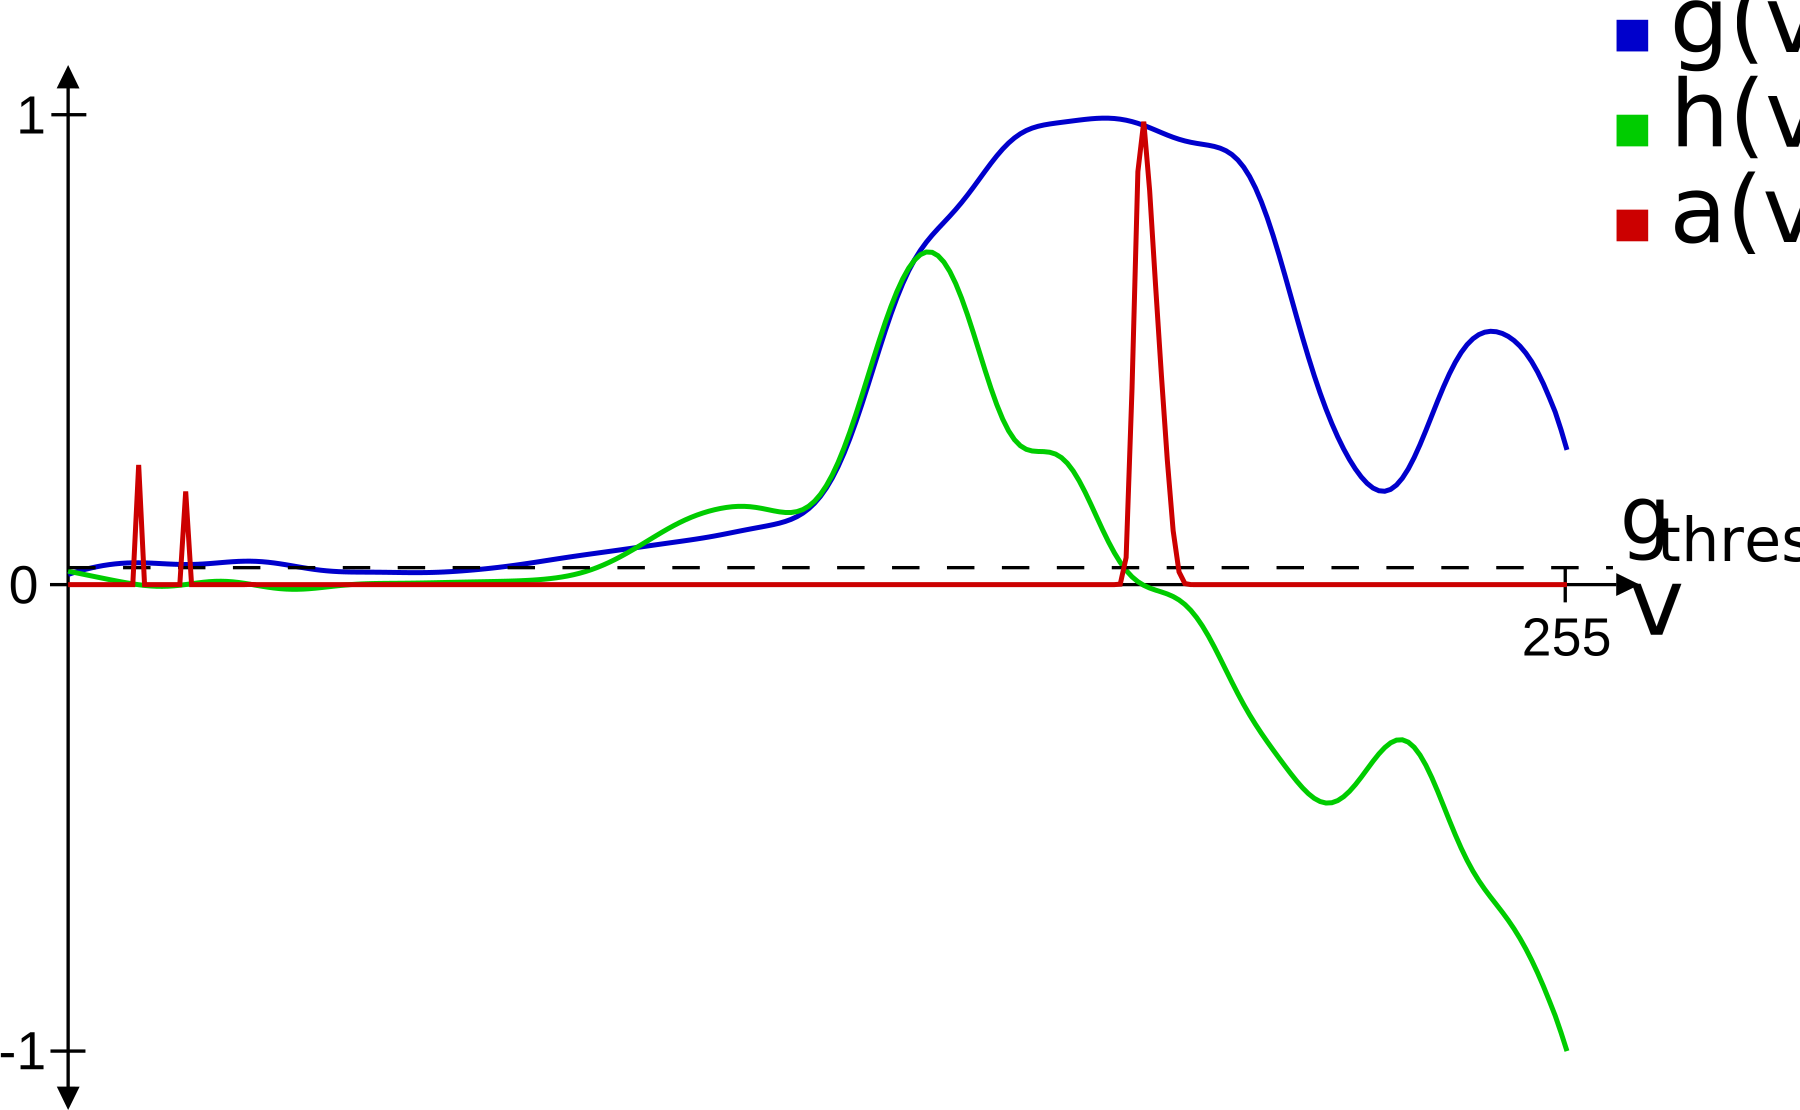
\includegraphics[width=0.65\textwidth]{images/r_vrep_so_2_kd_ft}
		\label{fig:r_vrep_2_kd}
	}
	\subfigure[Método proposto.]
	{
		\includegraphics[width=0.35\textwidth]{images/r_vrep_so_2_mine}
		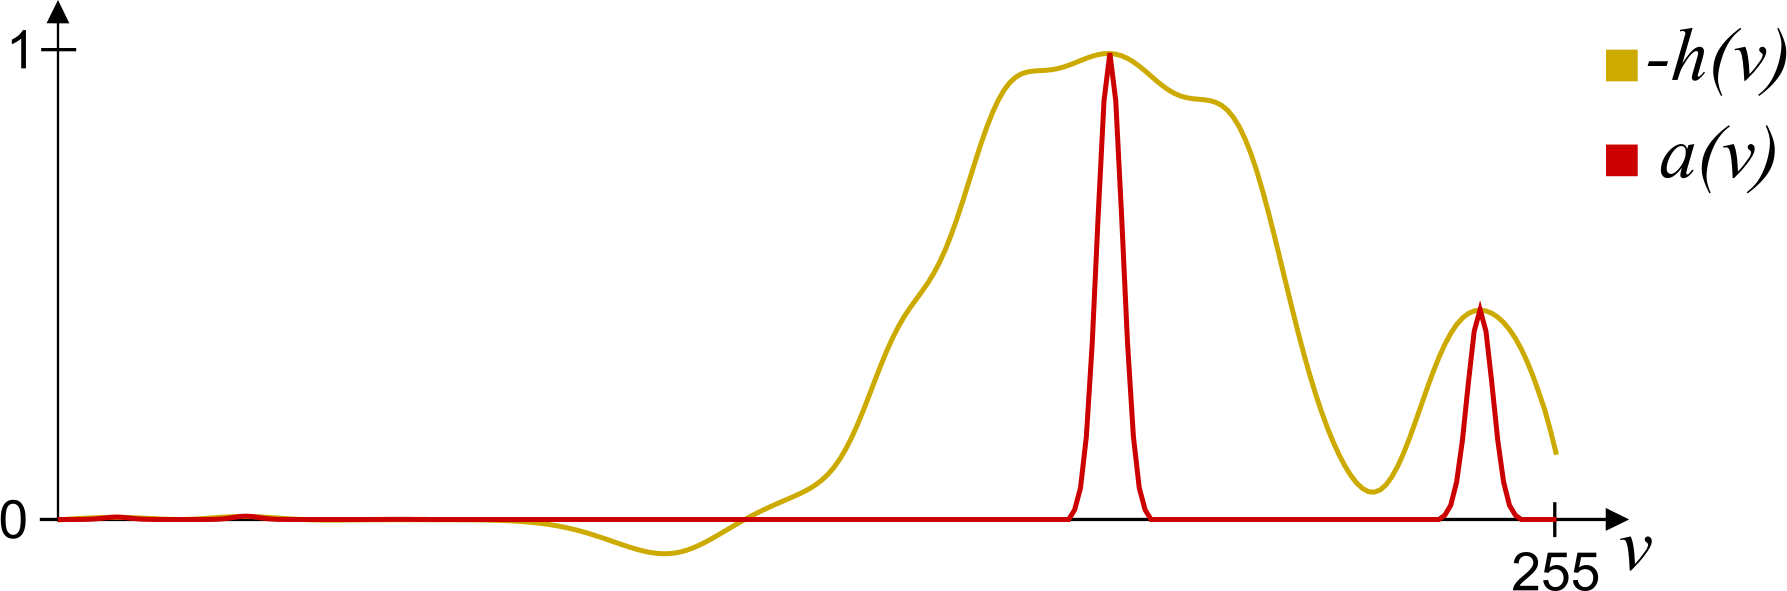
\includegraphics[width=0.65\textwidth]{images/r_vrep_so_2_mine_ft}			\label{fig:r_vrep_2_mine}
	}
	\caption{FT e visualização do volume de SO do modelo~A.}
	\label{fig:r_vrep_2}
\end{figure}

	Como mostra a Figura~\ref{fig:r_vrep_2}, nenhum método foi capaz de realçar todas as fronteiras. Utilizando \textit{Kindlmann e Durkin} obteve-se as fronteiras $ 1 $ e $ 4 $ enquanto com o método proposto nesta dissertação obteve-se as fronteiras $ 1 $, $ 3 $ e $ 4 $. O motivo pelo qual $ 4 $ é realçada com opacidade muito baixa é a estreita relação entre opacidade e amplitude de $ -h(v) $.
	
%%%%%%%%%%%%%%%%%%%%%%%%%%%%%%%%%% BOX SO %%%%%%%%%%%%%%%%%%%%%%%%%%%%%%%%%%%%%
\begin{figure}[h]
	\centering
	\frame{\includegraphics[width=0.5\textwidth]{images/r_box_so_slice}}
	\caption{Fatia do volume de SO do modelo B.}
\end{figure}

	A figura acima mostra uma fatia do volume de saturação de óleo do modelo B, que possui um poço injetor à esquerda e um produtor à direita. No lado esquerdo da fatia é possível perceber um cone, com sua base voltada para baixo. A parte interna do cone é preta e faz fronteira com seu contorno que possui uma tonalidade de cinza claro. Por sua vez, este contorno faz fronteira com o resto do volume em um tom de cinza mais escuro.
	
	Comparando a Figura~\ref{fig:r_box_so}~\ref{fig:r_box_so_kd} com a Figura~\ref{fig:r_box_so}~\ref{fig:r_box_so_mine} observa-se que o método de \textit{Kindlmann e Durkin} detectou o cone mais externo, enquanto o método proposto por esta dissertação detectou o cone mais interno. Ambas as visualizações auxiliam o usuário a compreender melhor o fluxo de óleo no reservatório. Porém, conceitualmente, o mais correto é o cone interno (detectado por esta dissertação em azul na Figura~\ref{fig:r_box_so}~\ref{fig:r_box_so_mine_ft}) por ser a fronteira mais forte, isto é, a que possui variação mais abrupta.

\begin{figure}[h]
	\centering
	\subfigure[Função de transferência pelo método de \textit{Kindlmann e Durkin}.]
	{
		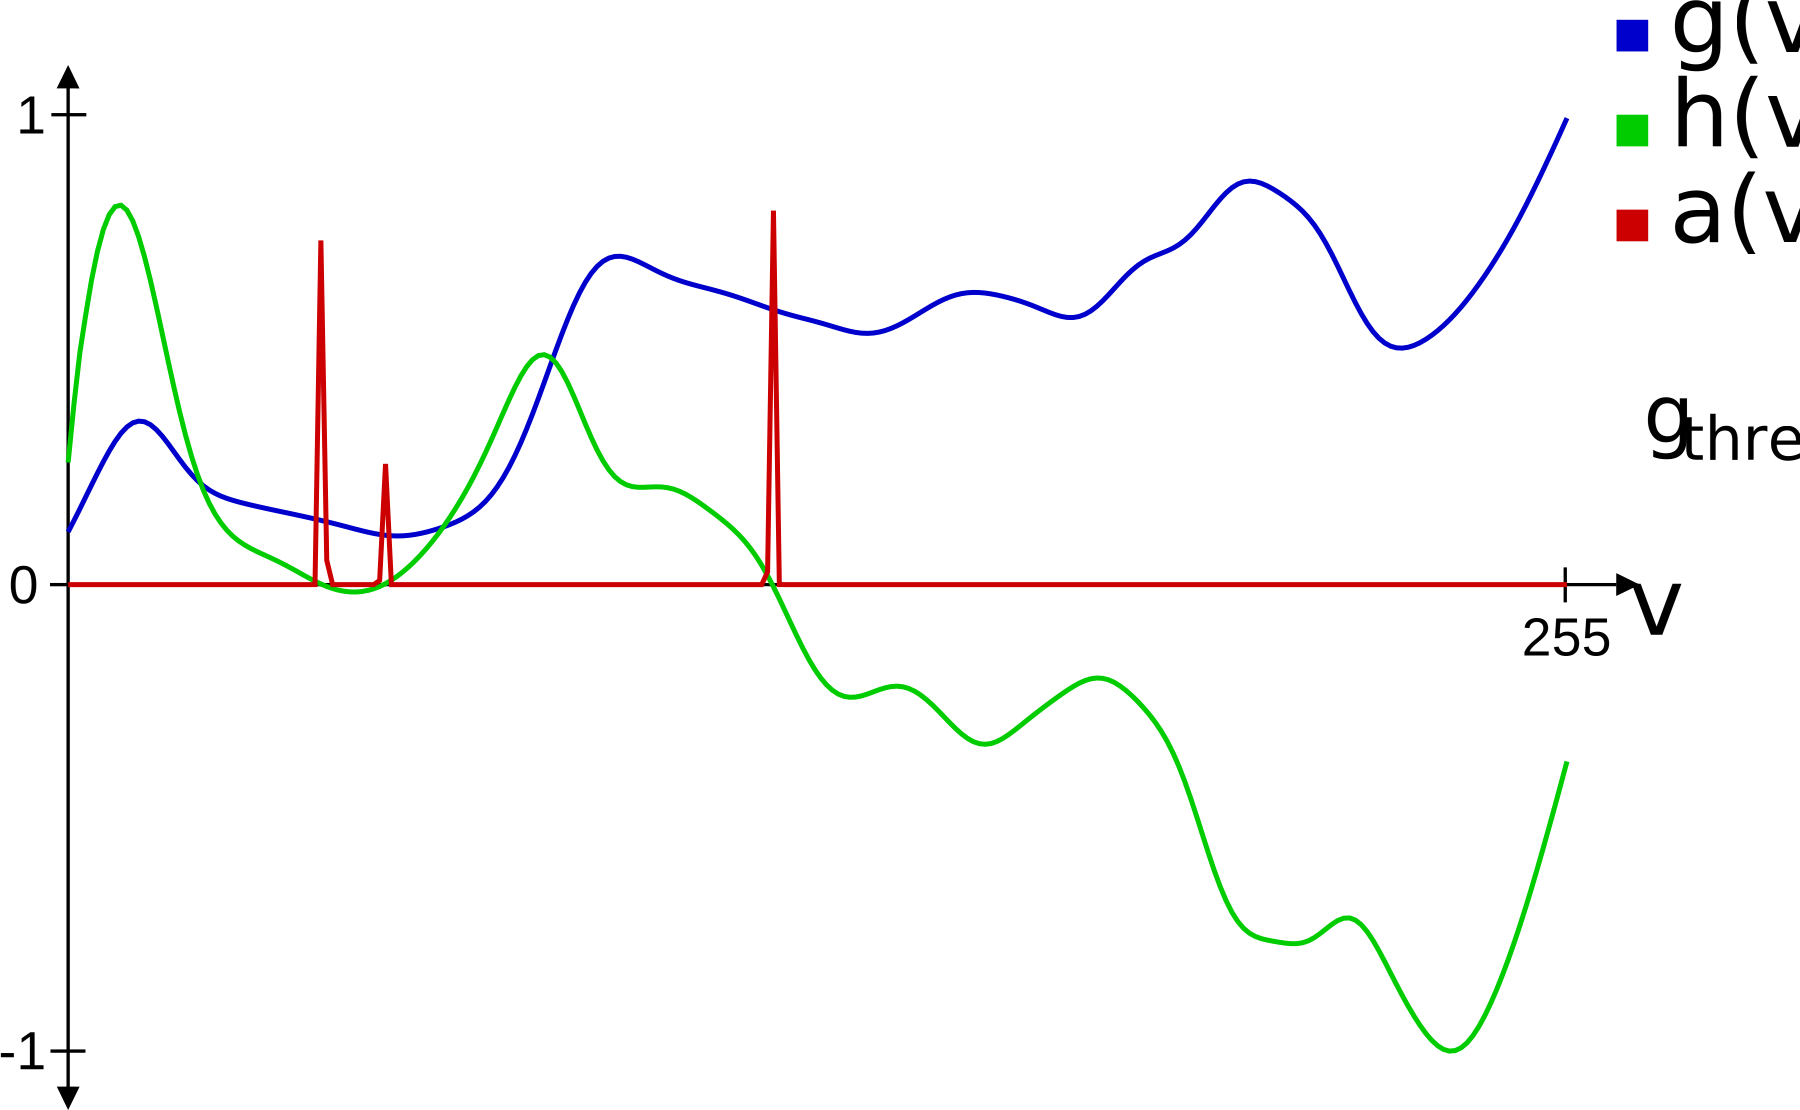
\includegraphics[width=0.7\textwidth]{images/r_box_so_kd_ft}
		\label{fig:r_box_so_kd_ft}
	}
	\subfigure[Visualização pela FT do método de \textit{Kindlmann e Durkin}.]
	{
		\includegraphics[width=0.7\textwidth]{images/r_box_so_kd}
		\label{fig:r_box_so_kd}
	}
	\subfigure[Função de transferência pelo método proposto.]
	{
		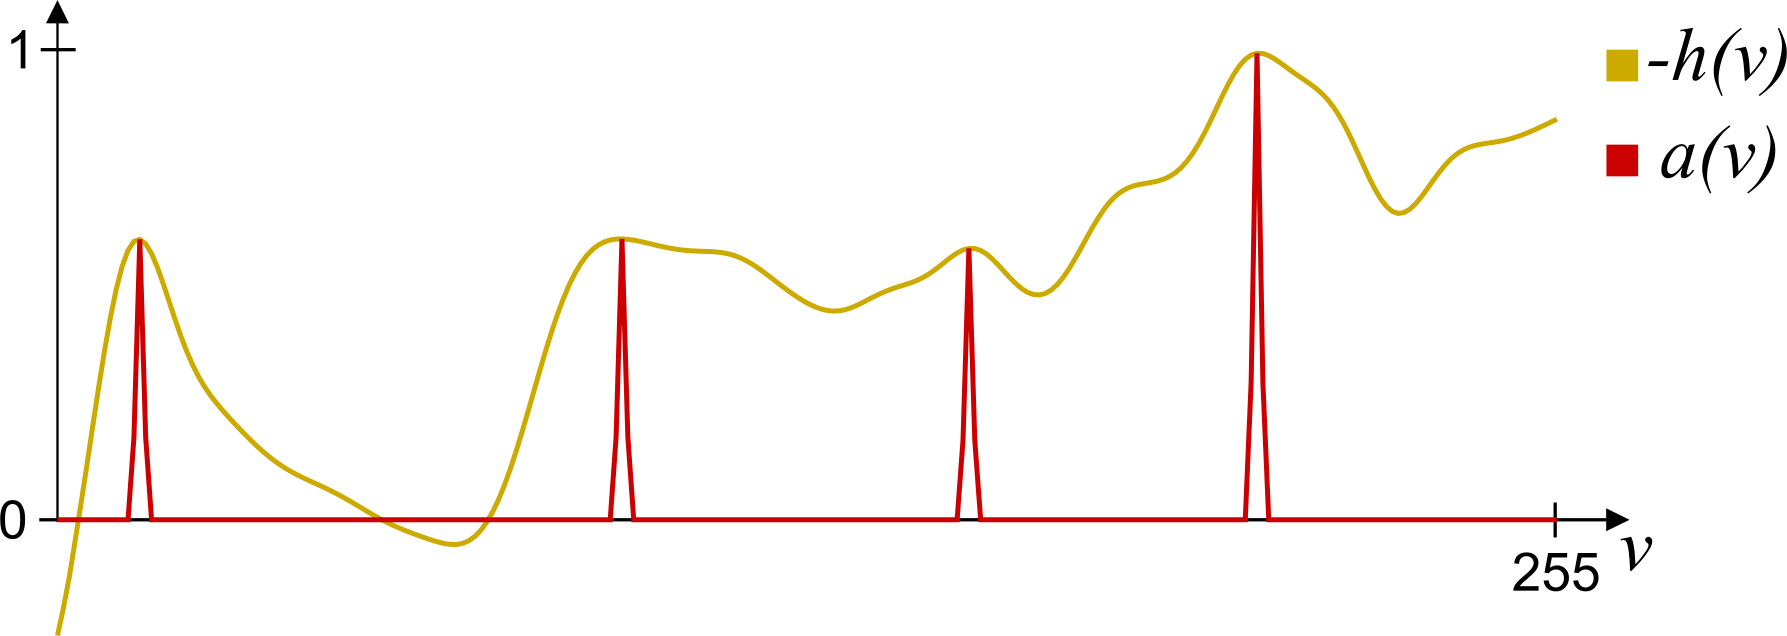
\includegraphics[width=0.7\textwidth]{images/r_box_so_mine_ft}			\label{fig:r_box_so_mine_ft}
	}
	\subfigure[Visualização pela FT do método proposto.]
	{
		\includegraphics[width=0.7\textwidth]{images/r_box_so_mine}	\label{fig:r_box_so_mine}
	}
	\caption{FT e visualização do volume de SO do modelo~B.}
	\label{fig:r_box_so}
\end{figure}
	
	Como esse volume é pequeno, falta resolução em sua fatia para discutir qual das fronteiras amarelas é a mais adequada. Contudo, pode-se ressaltar que ambos os métodos destacam fronteiras mais fracas que podem ser identificadas na fatia do volume, são elas: isosuperfície verde na Figura~\ref{fig:r_box_so}~\ref{fig:r_box_so_kd} e isosuperfície laranja na Figura~\ref{fig:r_box_so}~\ref{fig:r_box_so_mine}.

%%%%%%%%%%%%%%%%%%%%%%%%%%%%%%%%%% BOX SG %%%%%%%%%%%%%%%%%%%%%%%%%%%%%%%%%%%%%
\begin{figure}[h]
	\centering
	\frame{\includegraphics[width=0.5\textwidth]{images/r_box_sg_slice}}
	\caption{Fatia do volume de SG do modelo B.}
\end{figure}

	A figura acima mostra uma fatia do volume de saturação de gás (SG) do modelo B. Nela, nota-se que a fronteira principal se encontra entre o preto e o cinza claro.

\begin{figure}[h]
	\centering
	\subfigure[Método de \textit{Kindlmann e Durkin}.]
	{
		\includegraphics[width=0.8\textwidth]{images/r_box_sg_kd}
		\label{fig:r_box_sg_kd}
	}
	\subfigure[Método proposto.]
	{
		\includegraphics[width=0.8\textwidth]{images/r_box_sg_mine}	\label{fig:r_box_sg_mine}
	}
	\caption{Visualização do volume de SG do modelo~B.}
	\label{fig:r_box_sg}
\end{figure}

\begin{figure}[h]
	\centering
	\subfigure[Método de \textit{Kindlmann e Durkin}.]
	{
		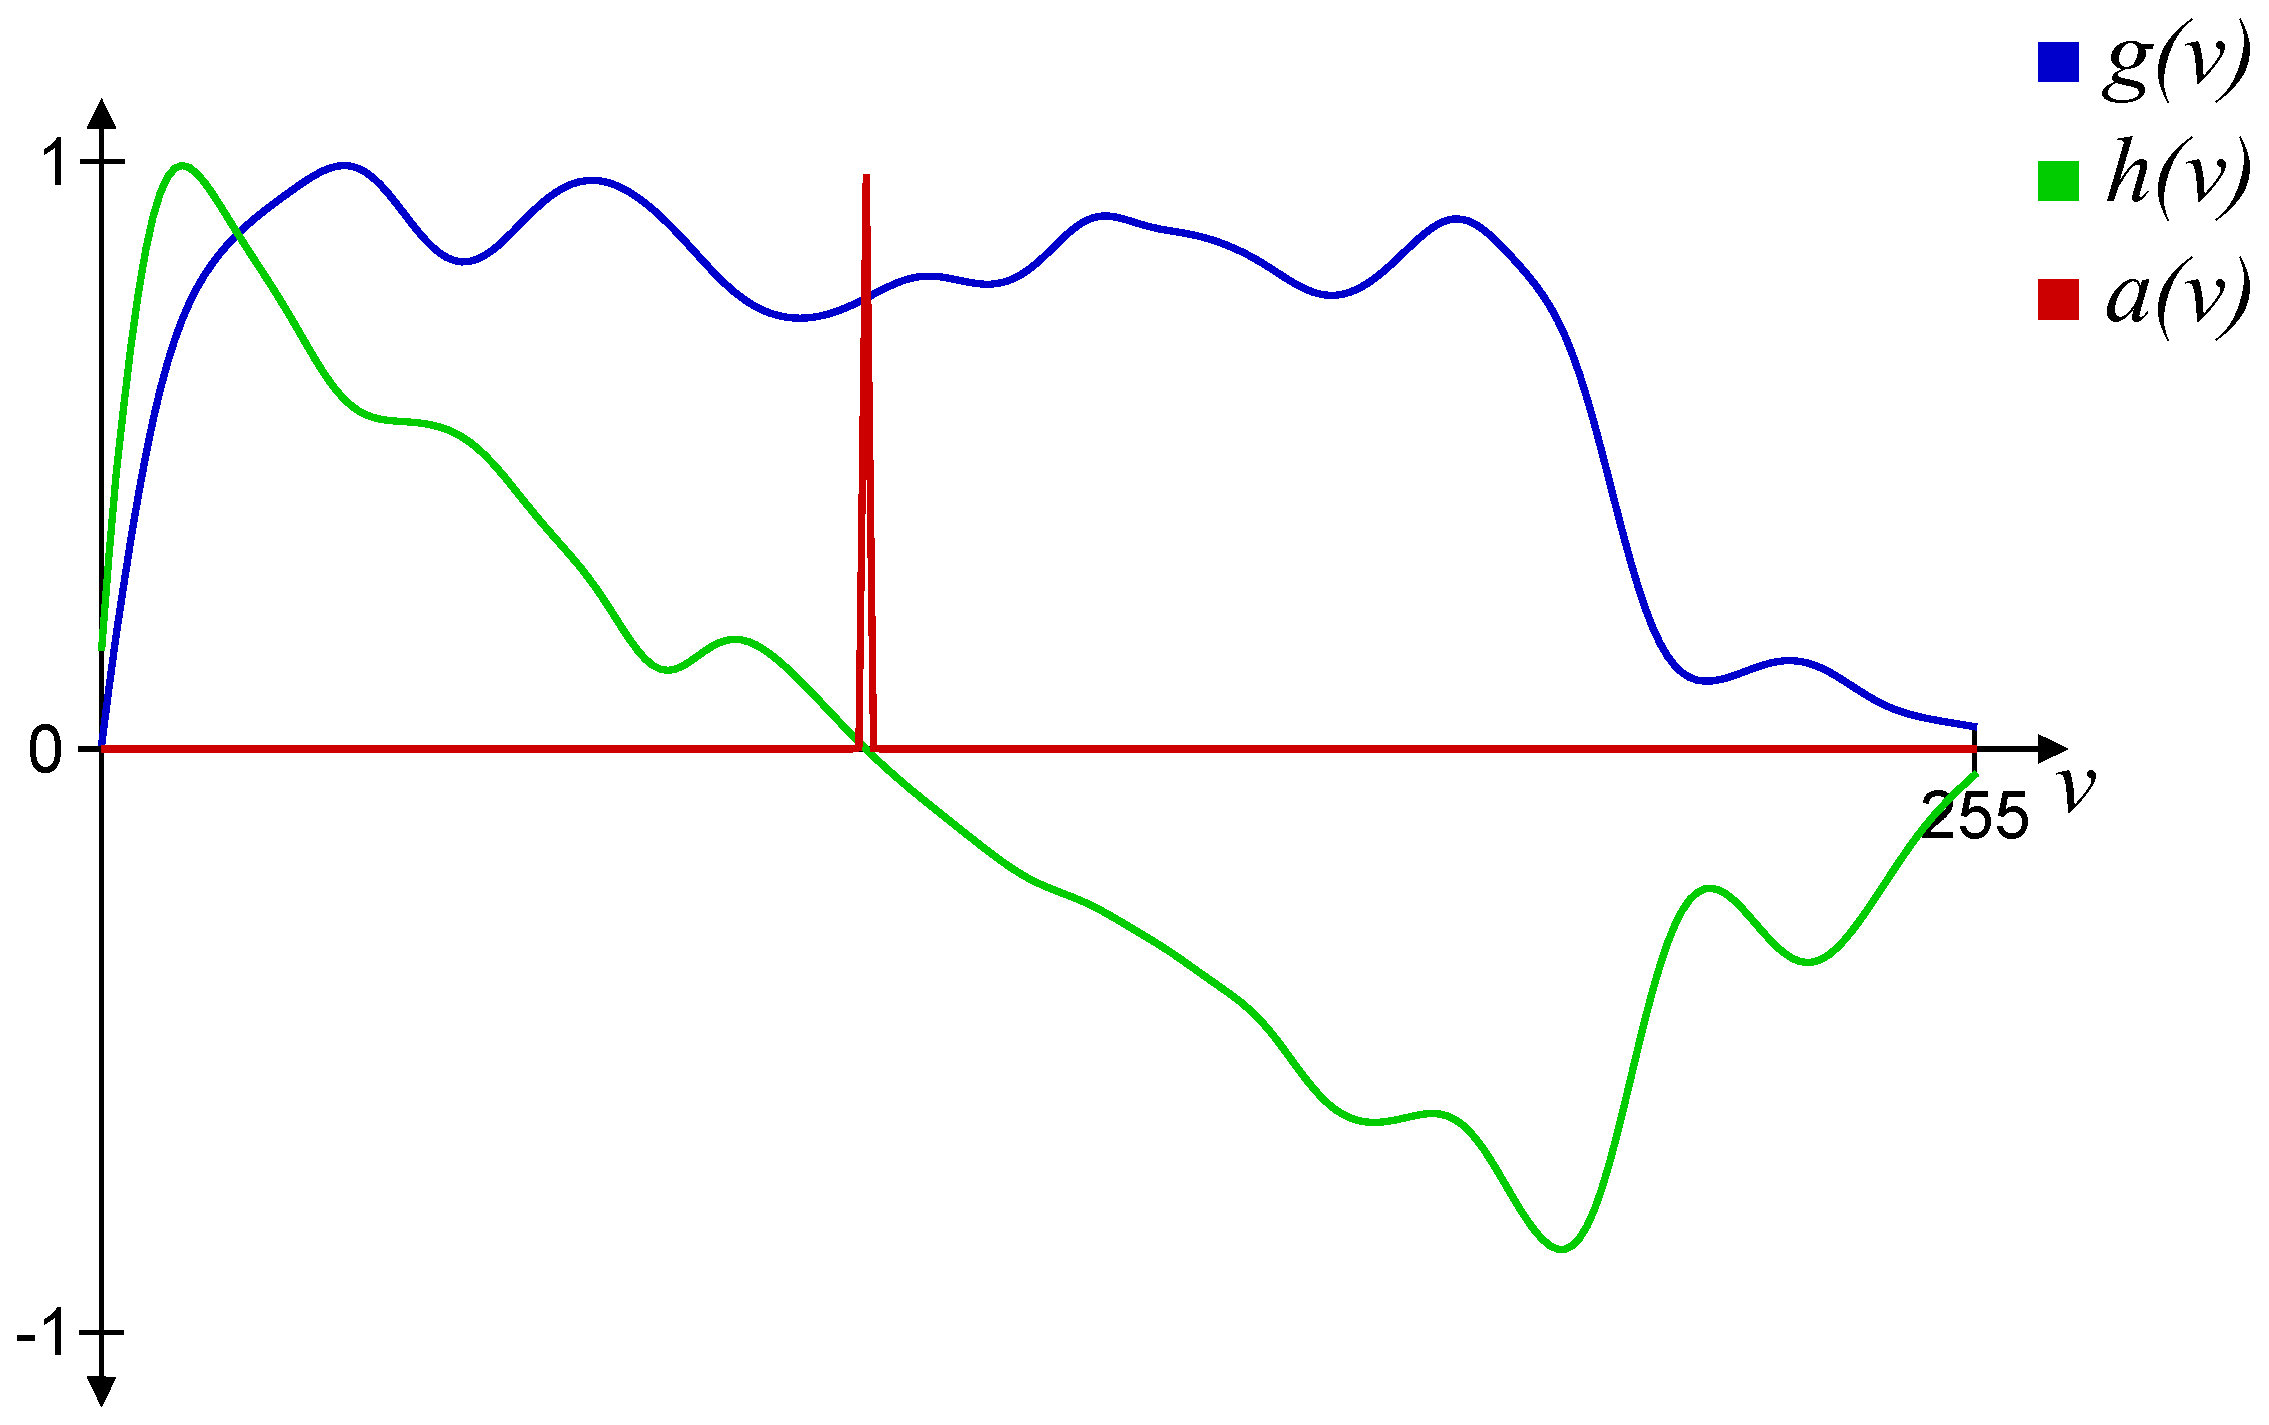
\includegraphics[width=0.7\textwidth]{images/r_box_sg_kd_ft}
		\label{fig:r_box_sg_kd_ft}
	}
	\subfigure[Método proposto.]
	{
		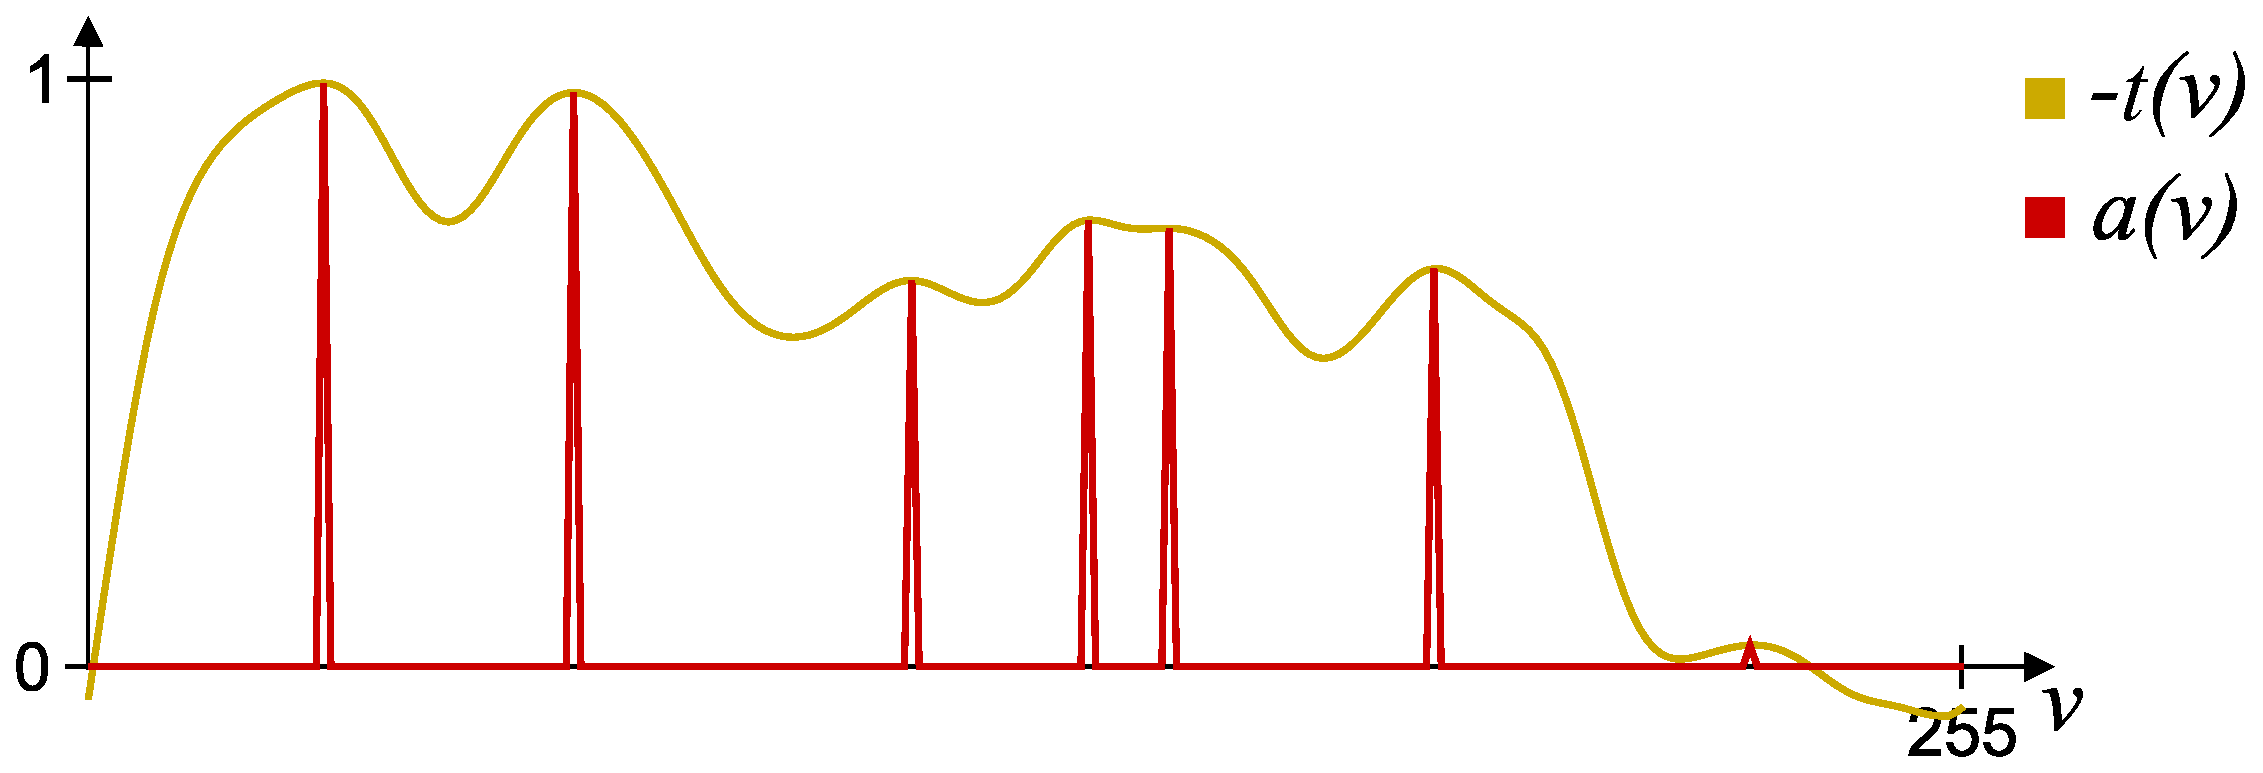
\includegraphics[width=0.7\textwidth]{images/r_box_sg_mine_ft}			\label{fig:r_box_sg_mine_ft}
	}
	\caption{Funções de transferência do volume de SG do modelo~B.}
	\label{fig:r_box_sg_ft}
\end{figure}

	Como pode ser observado na Figura~\ref{fig:r_box_sg}, o método de \textit{Kindlmann e Durkin} realça apenas a fronteira principal, enquanto o método proposto por esta dissertação destaca também a fronteira mais fraca, em vermelho na Figura~\ref{fig:r_box_sg}~\ref{fig:r_box_sg_mine}. Em contra partida, o método aqui proposto realça diversas isosuperfícies paralelas àquela que verdadeiramente identifica o centro da fronteira principal. Isso ocorre devido à pouca resolução do volume.
	
	Como a função de transferência proposta por esta dissertação não é proveniente de uma fórmula matemática que dependente dos valores da fronteira variarem de acordo com uma distribuição gaussiana, ela é capaz de identificar fronteiras menos borradas que a FT de \textit{Kindlmann e Durkin}~\cite{gordon}. Essa característica gera uma disparidade maior entre os métodos, na visualização de volumes com pouca resolução. Por um lado, permite que o método proposto identifique fronteiras mesmo que elas não se comportem de forma ideal, por outro, tende a encontrar fronteiras repetidas com deslocamento variado.

%%%%%%%%%%%%%%%%%%%%%%%%%%%%%%%%%% BOX SW %%%%%%%%%%%%%%%%%%%%%%%%%%%%%%%%%%%%%

	O volume a seguir ilustra bem a diferença entre os dois métodos, pois utilizando \textit{Kindlmann e Durkin} obtém-se apenas a fronteira mais forte, enquanto ao utilizar o método proposto nesta dissertação obtém-se algumas isosuperfícies paralelas à fronteira mais forte. Em compensação, o método proposto destaca também fronteiras mais fracas que podem ser claramente observadas a partir da fatia do volume, exibida na Figura~\ref{fig:r_box_sw_slice}. O volume em questão descreve a saturação de água (SW) do modelo B. Como pode ser observado, pelo menos três fronteiras são esperadas: preto-cinza claro, branco-cinza claro e cinza claro-cinza escuro. No entanto, como mostra a Figura~\ref{fig:r_box_sw}, apenas o método proposto por esta dissertação realça todas as fronteiras.
	
\begin{figure}[h]
	\centering
	\frame{\includegraphics[width=0.35\textwidth]{images/r_box_sw_slice}}
	\caption{Fatia do volume de SW do modelo B.}
	\label{fig:r_box_sw_slice}
\end{figure}

\begin{figure}[h]
	\centering
	\subfigure[Método de \textit{Kindlmann e Durkin}.]
	{
		\includegraphics[width=0.7\textwidth]{images/r_box_sw_kd}
		\label{fig:r_box_sw_kd}
	}
	\subfigure[Método de \textit{Kindlmann e Durkin}.]
	{
		\includegraphics[width=0.7\textwidth]{images/r_box_sw_kd_ft}
		\label{fig:r_box_sw_kd_ft}
	}
	\subfigure[Método proposto.]
	{
		\includegraphics[width=0.7\textwidth]{images/r_box_sw_mine}	\label{fig:r_box_sw_mine}
	}
	\subfigure[Método proposto.]
	{
		\includegraphics[width=0.7\textwidth]{images/r_box_sw_mine_ft}			\label{fig:r_box_sw_mine_ft}
	}
	\caption{Visualização e FT do volume de SW do modelo~B.}
	\label{fig:r_box_sw}
\end{figure}

%%%%%%%%%%%%%%%%%%%%%%%%%%%%%%%%%% Pituba %%%%%%%%%%%%%%%%%%%%%%%%%%%%%%%%%%%%%
\clearpage
	A figura abaixo mostra um momento da simulação da saturação de óleo de um modelo real de reservatório de petróleo, o Pituba. Essa visualização, feita pelo Geresim, incorpora uma função de transferência gerada automaticamente pelo método proposto nesta dissertação. Para este caso, não gerou-se uma função de opacidade mas uma função de peso, isto é, o valor da FT gerada multiplica cada coordenada rgb da FT de cores do Geresim. Assim, as fronteiras são realçadas através de cores mais claras, enquanto todo o resto do modelo possui tonalidades mais escuras.
	
\begin{figure}[h]
	\centering
	\includegraphics[width=1\textwidth]{images/pituba}
	\caption{Visualização do modelo Pituba através do Geresim, com uma FT gerada automaticamente pelo método descrito nesta dissertação.}
\end{figure}
	
	Nesta figura observa-se fronteiras (de cor laranja) circundando os poços de injeção (em azul). Essas regiões são consistentes com as fronteiras de avanço esperadas, já que é a partir dos poços de injeção de água que se formaram as interfaces entre a água e o óleo e, portanto, obtém a maior variação na saturação de óleo. Sendo assim, as fronteiras identificadas são bons indícios de onde se encontram as frentes de avanço.